\chapter[Advanced Data Representation]{Advanced Data\\ Representation}
\label{chap:advanced_data_representation}

% Position the image to the right of the heading.
\vspace{-9\baselineskip} % move up
\hfill
 \begin{minipage}{0.5\textwidth}
 \centering
 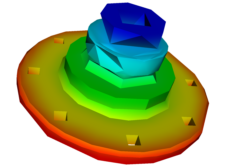
\includegraphics{VTKTextbook-158}\\
 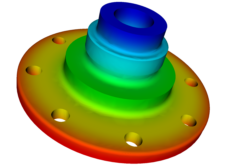
\includegraphics{VTKTextbook-157}
  \captionof*{figure}{\textit{Adaptive tessellation of higher-order cells.}}
 \end{minipage}
\vspace{2\baselineskip}

\firstletter{T}his chapter examines advanced topics in data representation.
Topics include topological and geometric relationships and computational methods for cells and datasets.

\section{Coordinate Systems}
\index{coordinate system|(}

We will examine three different coordinate systems: the global, dataset, and structured coordinate systems.
Figure \ref{fig:Figure8-1} shows the relationship between the global and dataset coordinate systems, and depicts the structured coordinate system.

\begin{figure}[!htb]
    \centering
    \begin{subfigure}{0.48\linewidth}
        \centering
        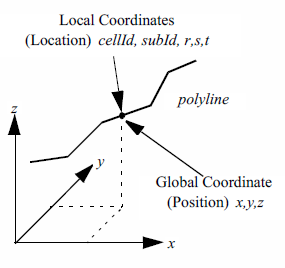
\includegraphics[width=\linewidth]{Figure8-1a}
        \caption*{}\label{fig:Figure8-1a}
    \end{subfigure}
    \hfill
    \begin{subfigure}{0.48\linewidth}
        \centering
        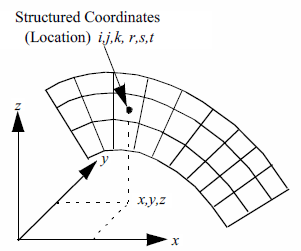
\includegraphics[width=\linewidth]{Figure8-1b}
        \caption*{}\label{fig:Figure8-1b}
    \end{subfigure}%
    \caption{Local and global coordinate systems.}
    \label{fig:Figure8-1}
\end{figure}


\subsection{Global Coordinate System}
\index{coordinate system!global|(}\index{global coordinate system|(}

The global coordinate system is a Cartesian, three-dimensional space. Each point is expressed as a triplet of values $(x,y,z)$ along the $x$, $y$, and $z$ axes.
This is the same system that was described in Chapter 3: \nameref{chap:computer_graphics_primer} (see \ref{sec:coordinate_systems}).
The global coordinate system is always used to specify dataset geometry (i.e., the point coordinates),and data attributes such as normals and vectors.
We will use the word ``position'' to indicate that we are using global coordinates.
\index{coordinate system!global|)}\index{global coordinate system|)}

\subsection{Dataset Coordinate System}
\index{coordinate system!dataset|(}\index{dataset!coordinate system|(}

The dataset, or local, coordinate system is based on combined topological and geometric coordinates. The topological coordinate is used to identify a particular cell (or possibly a subcell), and the geometric coordinate is used to identify a particular location within the cell. Together they uniquely specify a location in the dataset. Here we will use the word ``location'' to refer to local or dataset coordinates.

The topological coordinate is an ``id'': a unique, nonnegative integer number referring to either a dataset point or cell. For a composite cell, we use an additional ``sub-id'' to refer to a particular primary cell that composes the composite cell. The sub-id is also unique and nonnegative. The id and sub-id together select a particular primary cell.

To specify a location within the primary cell, we use geometric coordinates. These geometric coordinates, or parametric coordinates, are coordinates ``natural'' or canonical to the particular topology and dimension of a cell.

We can best explain local coordinates by referring to an example. If we consider the polyline cell type shown in Figure \ref{fig:Figure8-2}, we can specify the position of a point by indicating 1) the polyline cell id, 2) the primary cell (i.e., line) sub-id and 3) the parametric coordinate of the line. Because the line is one-dimensional, the natural or parametric coordinate is based on the one-dimensional parameter r. Then any point along the line is given by a linear combination of the two end points of the line $x_i$ and $x_{i+1}$

\begin{equation}\label{eq:8.1}
x(r) = (1 - r) x_i + r x_{i + 1}
\end{equation}
\myequations{Parametric equation of a line.}

where the parametric coordinate $r$ is constrained between $(0,1)$. In this equation we are assuming that the sub-id is equal to $i$.

The number of parametric coordinates corresponds to the topological dimension of the cell. Three-dimensional cells will be characterized by the three parametric coordinates $(r, s, t)$. For cells of topological order less than three, we will ignore the last $(3 - n)$ parametric coordinates, where $n$ is the topological order of the cell. For convenience and consistency, we also will constrain each parametric coordinate to range between $(0,1)$.

Every cell type will have its own parametric coordinate system. Later in this chapter we will describe the parametric coordinate systems in detail. But first we will examine another coordinate system, the structured coordinate system.
\index{coordinate system!dataset|)}\index{dataset!coordinate system|)}

\subsection{Structured Coordinate System}
\label{subsec:structured_coordinate_system}
\index{coordinate system!structured|(}

Many dataset types are structured. This includes image data and structured grids. Because of their inherent structure, they have their own natural coordinate system. This coordinate system is based on the $i-j-k$ indexing scheme that we touched on in Chapter 5: \nameref{chap:basic_data_representation} (see``Image Data'' on page \pageref{subsec:image_data}).

The structured coordinate system is a natural way to describe components of a structured dataset. By fixing some indices, and allowing the others to vary within a limited range, we can specify points, lines, surfaces, and volumes. For example, by fixing the $i$ index $i = i_0$, and allowing the $j$ and $k$ indices to range between their minimum and maximum values, we specify a surface. If we fix three indices, we specify a point, if we fix two indices, we specify a line, and if we allow three indices to vary, we specify a volume (or sub-volume). The structured coordinate system is generally used to specify a region of interest (or ROI). The region of interest is an area that we want to visualize, or to operate on.

There is a simple relationship between the point and cell id of the dataset coordinate system and the structured coordinate system. To obtain a point id $p_\text{id}$ given the indices $(i_p, j_p, k_p)$ and dimensions $(n_x, n_y, n_z)$ we use

\begin{equation}\label{eq:8.2}
p_\text{id} = i_p +j_p n_x + k_p n_y
\end{equation}
\myequations{Obtaining a point id.}

with $0 \leq i_p \leq n_x, 0 \leq j_p \leq n_y, 0 \leq k_p \leq n_z$. (We can use this id to index into an array of points or point attribute data.) This equation implicitly assumes an ordering of the points in topological space. Points along the $i$ axis vary fastest, followed by the $j$ and then the $k$ axes. A similar relationship exists for cell id's

\begin{equation}\label{eq:8.3}
\text{cell}_\text{id} = i_p + j_p (n_x - 1) + k_p (n_x - 1)(n_y - 1)
\end{equation}
\myequations{Obtaining a cell id.}

Here we've taken into account that there are one fewer cells along each topological axes than there are points.
\index{coordinate system!structured|)}
\index{coordinate system|)}

\section{Interpolation Functions}
\label{sec:interpolation_functions}
\index{interpolation function|(}

Computer visualization deals with discrete data. The data is either supplied at a finite number of points or created by sampling continuous data at a finite number of points. But we often need information at positions other than these discrete point locations. This may be for rendering or for sub-sampling the data during algorithm execution. We need to interpolate data from known points to some intermediate point using \emph{interpolation functions}.

Interpolation functions relate the values at cell points to the interior of the cell. Thus, we assume that information is defined at cell points, and that we must interpolate from these points. We can express the result as a weighted average of the data values at each cell point.

\begin{figure}[!htb]
    \centering
    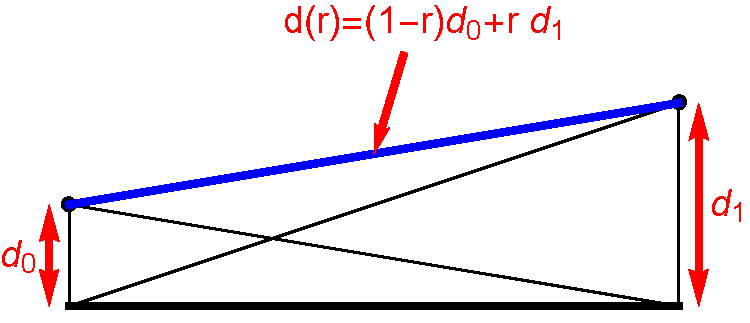
\includegraphics[width=0.98\textwidth]{Figure8-2}\\
    \caption{Interpolation is a linear combination of local interpolation functions. Interpolation functions are scaled by data values at cell points.}\label{fig:Figure8-2}
\end{figure}

\subsection{General Form}

To interpolate\index{interpolate} data from the cell points $p_i$ to a point $p$ that is inside the cell, we need three pieces of information:

\begin{itemize}

    \item the data values at each cell point,

    \item the parametric coordinates of the point $p$ within the cell, and

    \item the cell type including interpolation functions.

\end{itemize}

Given this information, the interpolation functions are a linear combination of the data values at the cell points

\begin{equation}\label{eq:8.4}
d = \sum_{i = 0}^{n - 1}W_i\,  d_i
\end{equation}
\myequations{Linear combination of data values at each cell point.}

where $d$ is the data value at the interior cell location $(r,s,t)$, $d_i$ is the data value at the $i^{th}$ cell point, and $W_i$ is a weight at the $i^{th}$ cell point. The interpolation weights are functions of the parametric coordinates $W_i = W(r,s,t)$. In addition, because we want $d = d_i$ when the interior point coincides with a cell point, we can place additional constraints on the weights

\begin{equation}\label{eq:8.5}
W_i = 1, W_{j \neq i} = 0 \quad \text{when} \quad p = p_i
\end{equation}
\myequations{Weighting constraints.}

We also desire the interpolated data value $d$ to be no smaller than the minimum $d_i$ and no larger than the maximum $d_i$. Thus the weights should also satisfy

\begin{equation}\label{eq:8.6}
\sum W_i = 1, \quad 0 \leq W_i \leq 1
\end{equation}
\myequations{Additional weighting constraints.}

The interpolation functions are of a characteristic shape. They reach their maximum value $W_i = 1$ at cell point $p_i$, and are zero at all other points. Examining Equation \ref{eq:8.1}, we draw Figure \ref{fig:Figure8-2} and see that each interpolation function has the shape of a peaked ``hat'', and that interpolation is a linear combination of these hat functions, scaled by the data value at each point.

Equation \ref{eq:8.4} is the general form for cell interpolation. It is used to interpolate any data value defined at the cell points to any other point within the cell. We have only to define the specific interpolation functions $W_i$ for each cell type.

\subsection{Specific Forms}

Each cell type has its own interpolation functions. The weights $W_i$ are functions of the parametric coordinates $r$, $s$, and $t$. In this section we will define the parametric coordinate system and interpolation function for each primary cell type. Composite cells use the interpolation functions and parametric coordinates of their composing primary cells. The only difference in coordinate system specification between primary and composite cells is that composite cells use the additional sub-id to specify a particular primary cell.

\begin{description}

    \begin{figure}[!htb]
        \centering
        \begin{subfigure}{0.48\linewidth}
            \centering
            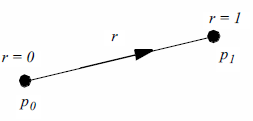
\includegraphics[width=\linewidth]{Figure8-3}
            \caption*{}
        \end{subfigure}
        \hfill
        \begin{subfigure}{0.48\linewidth}
            \centering
            \begin{equation*}
            \begin{array}{lll}
                W_0 &=& 1-r \\
                W_1 &=& r
            \end{array}
            \end{equation*}
        \end{subfigure}%
        \caption{Parametric coordinate system and interpolation functions for a line.}
        \label{fig:Figure8-3}
    \end{figure}

    \begin{figure}[!htb]
        \centering
        \begin{subfigure}{0.48\linewidth}
            \centering
            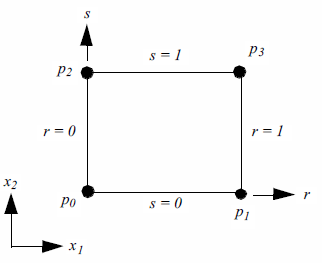
\includegraphics[width=\linewidth]{Figure8-4}
            \caption*{}
        \end{subfigure}
        \hfill
        \begin{subfigure}{0.48\linewidth}
            \centering
            \begin{equation*}
            \begin{array}{lll}
            W_0 &=& (1-r)(1 - s) \\
            W_1 &=& r(1 - s) \\
            W_2 &=& (1 - r)s \\
            W_3 &=& r s
            \end{array}
            \end{equation*}
        \end{subfigure}%
        \caption{Parametric coordinate system and interpolation functions for a pixel.}
        \label{fig:Figure8-4}
    \end{figure}

    \begin{figure}[!htb]
        \centering
        \begin{subfigure}{0.48\linewidth}
            \centering
            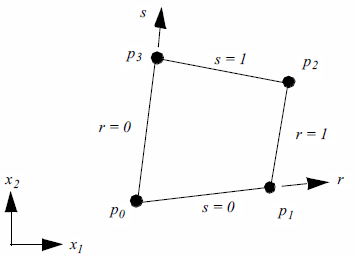
\includegraphics[width=\linewidth]{Figure8-5}
            \caption*{}
        \end{subfigure}
        \hfill
        \begin{subfigure}{0.48\linewidth}
            \centering
            \begin{equation*}
            \begin{array}{lll}
            W_0 &=& (1-r)(1 - s) \\
            W_1 &=& r(1 - s) \\
            W_2 &=& r s \\
            W_3 &=& (1 - r)s
            \end{array}
            \end{equation*}
        \end{subfigure}%
        \caption{Parametric coordinate system and interpolation functions for a quadrilateral.}
        \label{fig:Figure8-5}
    \end{figure}

%\clearpage
    \begin{figure}[!htb]
        \centering
        \begin{subfigure}{0.48\linewidth}
            \centering
            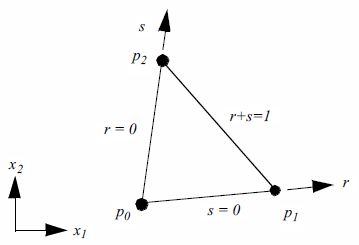
\includegraphics[width=\linewidth]{Figure8-6}
            \caption*{}
        \end{subfigure}
        \hfill
        \begin{subfigure}{0.48\linewidth}
            \centering
            \begin{equation*}
            \begin{array}{lll}
            W_0 &=& 1 - r - s \\
            W_1 &=& r \\
            W_2 &=& s
            \end{array}
            \end{equation*}
        \end{subfigure}%
        \caption{Parametric coordinate system and interpolation functions for a triangle.}
        \label{fig:Figure8-6}
    \end{figure}

    \begin{figure}[!htb]
        \centering
        \begin{subfigure}{0.48\linewidth}
            \centering
            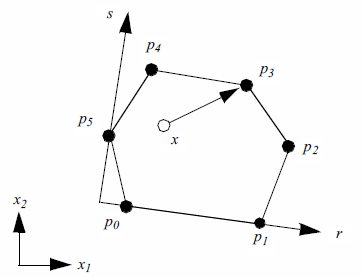
\includegraphics[width=\linewidth]{Figure8-7}
            \caption*{}
        \end{subfigure}
        \hfill
        \begin{subfigure}{0.48\linewidth}
            \centering
            \begin{equation*}
            \begin{array}{lll}
            W_i &=& \dfrac{r_i^{-2}}{\sum r_i^{-2}} \\ \\
            r_i &=& \vert p_i - x \vert
            \end{array}
            \end{equation*}
        \end{subfigure}%
        \caption{Parametric coordinate system and interpolation functions for a polygon.}
        \label{fig:Figure8-7}
    \end{figure}

    \begin{figure}[!htb]
        \centering
        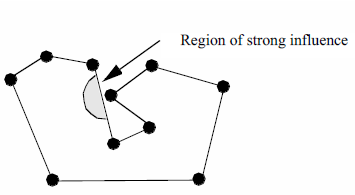
\includegraphics[width=0.48\textwidth]{Figure8-8}\\
        \caption{Potential problem with distance-based interpolation functions.}\label{fig:Figure8-8}
    \end{figure}

%\clearpage
    \begin{figure}[!htb]
        \centering
        \begin{subfigure}{0.48\linewidth}
            \centering
            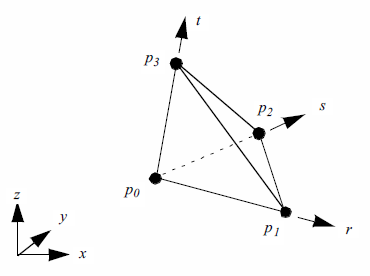
\includegraphics[width=\linewidth]{Figure8-9}
            \caption*{}
        \end{subfigure}
        \hfill
        \begin{subfigure}{0.48\linewidth}
            \centering
            \begin{equation*}
            \begin{array}{lll}
            W_0 &=& 1 - r - s - t \\
            W_1 &=& r \\
            W_2 &=& s \\
            W_3 &=& t
            \end{array}
            \end{equation*}
        \end{subfigure}%
        \caption{Parametric coordinate system and interpolation functions for a tetrahedron.}
        \label{fig:Figure8-9}
    \end{figure}

    \begin{figure}[!htb]
        \centering
        \begin{subfigure}{0.48\linewidth}
            \centering
            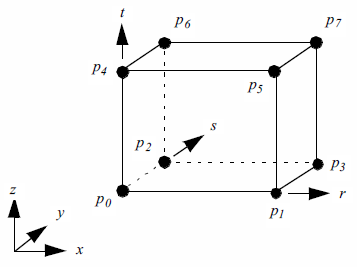
\includegraphics[width=\linewidth]{Figure8-10}
            \caption*{}
        \end{subfigure}
        \hfill
        \begin{subfigure}{0.48\linewidth}
            \centering
            \begin{equation*}
            \begin{array}{lll}
            W_0 &=& (1 - r)(1 - s)(1 - t) \\
            W_1 &=& r (1-s)(1 -t) \\
            W_2 &=& (1-r)s(1-t) \\
            W_3 &=& rs(1 - t) \\
            W_4 &=& (1 - r)(1 - s) t \\
            W_5 &=& r (1-s)t \\
            W_6 &=& (1 - r)s t \\
            W_7 &=& r s t
            \end{array}
            \end{equation*}
        \end{subfigure}%
        \caption{Parametric coordinate system and interpolation functions for a tetrahedron.}
        \label{fig:Figure8-10}
    \end{figure}

    \item[Vertex.] Vertex cells do not require parametric coordinates or interpolation functions since they are zero-dimensional. The single weighting function is $W_0 = 1$.

    \item[Line.] Figure \ref{fig:Figure8-3} shows the parametric coordinate system and interpolation functions for a line.The line is described using the single parametric coordinate $r$.

    \item[Pixel.] Figure \ref{fig:Figure8-4} shows the parametric coordinate system and interpolation functions for a pixel cell type. The pixel is described using the two parametric coordinates $(r,s)$. Note that the pixel edges are constrained to lie parallel to the global coordinate axes. These are often referred to as \emph{bilinear interpolation}\index{bilinear interpolation} functions.

    \item[Quadrilateral.] Figure \ref{fig:Figure8-5} shows the parametric coordinate system and interpolation functions for a quadrilateral cell type. The quadrilateral is described using the two parametric coordinates $(r,s)$.

    \item[Triangle.] Figure \ref{fig:Figure8-6} shows the parametric coordinate system and interpolation functions for a triangle cell type. The triangle is characterized using the two parametric coordinates $(r,s)$.


%\clearpage
    \begin{figure}[!htb]
        \centering
        \begin{subfigure}{0.48\linewidth}
            \centering
            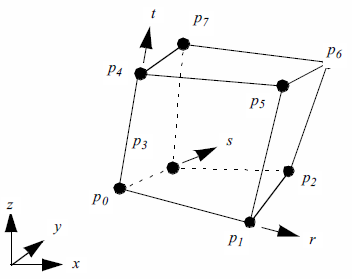
\includegraphics[width=\linewidth]{Figure8-11}
            \caption*{}
        \end{subfigure}
        \hfill
        \begin{subfigure}{0.48\linewidth}
            \centering
            \begin{equation*}
            \begin{array}{lll}
            W_0 &=& (1 - r)(1 - s)(1 - t) \\
            W_1 &=& r (1-s)(1 -t) \\
            W_2 &=& rs (1-t) \\
            W_3 &=& (1-r)s(1 - t) \\
            W_4 &=& (1 - r)(1 - s) t \\
            W_5 &=& r (1-s)t \\
            W_6 &=& rs t \\
            W_7 &=& (1-r)st
            \end{array}
            \end{equation*}
        \end{subfigure}%
        \caption{Parametric coordinate system and interpolation functions for a hexahedron.}
        \label{fig:Figure8-11}
    \end{figure}

    \begin{figure}[!htb]
        \centering
        \begin{subfigure}{0.48\linewidth}
            \centering
            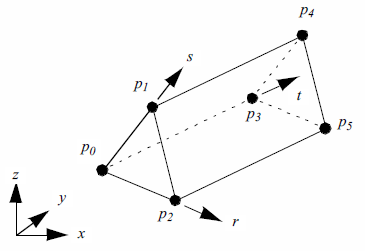
\includegraphics[width=\linewidth]{Figure8-12}
            \caption*{}
        \end{subfigure}
        \hfill
        \begin{subfigure}{0.48\linewidth}
            \centering
            \begin{equation*}
            \begin{array}{lll}
            W_0 &=& (1 - r - s)(1 - t) \\
            W_1 &=& r (1-t) \\
            W_2 &=& s (1 - t) \\
            W_3 &=& (1 - r - s)t \\
            W_4 &=& r t \\
            W_5 &=& s t
            \end{array}
            \end{equation*}
        \end{subfigure}%
        \caption{Parametric coordinate system and interpolation functions for a wedge.}
        \label{fig:Figure8-12}
    \end{figure}

    \item[Polygon.] Figure \ref{fig:Figure8-7} shows the parametric coordinate system and interpolation functions for a polygon cell type. The polygon is characterized using the two parametric coordinates $(r,s)$. The parametric coordinate system is defined by creating a rectangle oriented along the first edge of the polygon. The rectangle also must bound the polygon.

    The polygon poses a special problem since we do not know how many vertices define the polygon. As a result, it is not possible to create general interpolation functions in the fashion of the previous functions we have seen. Instead, we use a function based on weighted distance squared from each polygon vertex.

    The weighted distance squared interpolation functions work well in practice. However, there are certain rare cases where points topologically distant from the interior of a polygon have an undue effect on the polygon interior (Figure \ref{fig:Figure8-8}). These situations occur only if the polygon is concave and wraps around on itself.

%\clearpage
    \begin{figure}[!htb]
        \centering
        \begin{subfigure}{0.48\linewidth}
            \centering
            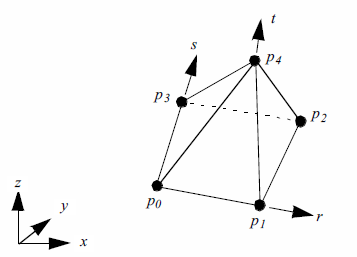
\includegraphics[width=\linewidth]{Figure8-13}
            \caption*{}
        \end{subfigure}
        \hfill
        \begin{subfigure}{0.48\linewidth}
            \centering
            \begin{equation*}
            \begin{array}{lll}
            W_0 &=& (1-r)(1-s)(1-t) \\
            W_1 &=& r(1-s)(1-t) \\
            W_2 &=& r s (1-t) \\
            W_3 &=& (1-r)s(1-t) \\
            W_4 &=& t
            \end{array}
            \end{equation*}
        \end{subfigure}%
        \caption{Parametric coordinate system and interpolation functions for a pyramid.}
        \label{fig:Figure8-13}
    \end{figure}

    \begin{figure}[!htb]
        \centering
        \begin{subfigure}{0.48\linewidth}
            \centering
            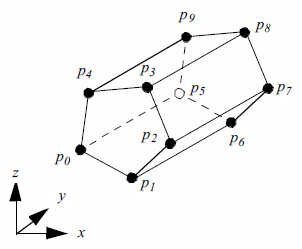
\includegraphics[width=\linewidth]{Figure8-14a}
            \caption*{}
        \end{subfigure}
        \hfill
        \begin{subfigure}{0.48\linewidth}
            \centering
            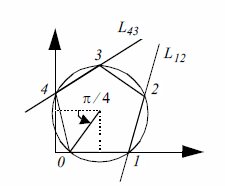
\includegraphics[width=\linewidth]{Figure8-14b}
            \caption*{}
        \end{subfigure}
        \hfill
        \begin{subfigure}{0.48\linewidth}
            \centering
            \begin{equation*}
            \begin{array}{lll}
            W_0 &=& -N(-As + Br - C)(Bs-Ar-C)(t - 1) \\
            W_1 &=& N(Ds+Dr-E)(Fs-Gr-H)(t-1) \\
            W_2 &=& -N(Bs -Ar -C)(-Gs-Fr+H)(t - 1)\\
            W_3 &=& N(-As + Br -C)(Fs + Gr - H)(t - 1) \\
            W_4 &=& -N(-Gs - Fr + H)(Ds + Dr - E)(t - 1) \\
            W_5 &=& N(-As +Br - C)(Bs -Ar -C)t \\
            W_6 &=& -N(Ds + Dr - E)(Fs + Gr - H)t\\
            W_7 &=& N(Bs - Ar -C)(-Gs -Fr + H)t \\
            W_8 &=& -N(-As + Br -C)(Fs + Gr - H)t \\
            W_9 &=& N(-Gs - Fr + H)(Ds + Dr -E)t
            \end{array}
            \end{equation*}
        \end{subfigure}%
        \hfill
        \begin{subfigure}{0.48\linewidth}
            \centering
            The points $P_i(x_i, y_i)$ on the pentagon are defined by:
            \begin{equation*}
            \begin{array}{lll}
            x_i &=& \dfrac{1}{2}\left(1 +\cos\left(\dfrac{5\pi}{4} + i \dfrac{2\pi}{5}\right)\right) \\ \\
            y_i &=& \dfrac{1}{2}\left(1 +\sin\left(\dfrac{5\pi}{4} + i \dfrac{2\pi}{5}\right)\right) \\ \\
            i &\in& \lbrace 0, 1, 2, 3, 4 \rbrace
            \end{array}
            \end{equation*}
            Constants:
            \begin{equation*}
            \begin{array}{lll}
            A &=& x_2 - x_1 \\
            B &=& y_2 - y_1 \\
            C &=& x_1 y_2 - x_2 y_1 \\
            D &=& x_2 - x_3 \\
            E &=& x_2 y_3 - x_3 y_2 \\
            F &=& x_0 - x_4 \\
            G &=& y_4 - y_0 \\
            H &=& x_0 y_4 - x_4 y_0
            \end{array}
            \end{equation*}
        \end{subfigure}%
        \caption{Parametric coordinate system and interpolation functions for a pentagonal prism.}
        \label{fig:Figure8-14}
    \end{figure}

%\clearpage
    \begin{figure}[!htb]
        \centering
        \begin{subfigure}{0.48\linewidth}
            \centering
            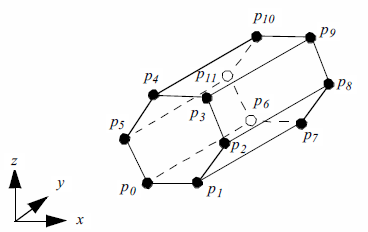
\includegraphics[width=\linewidth]{Figure8-15}
            \caption*{}
        \end{subfigure}
        \hfill
        \begin{subfigure}{0.48\linewidth}
            \centering
            \begin{equation*}
            \begin{array}{lll}
            \alpha &=& \dfrac{\sqrt{3}}{4} + \dfrac{1}{2} \\ \\
            \beta &=& \dfrac{1}{2} - \dfrac{\sqrt{3}}{4}, \alpha + \beta = 1
            \end{array}
            \end{equation*}
        \end{subfigure}
        \hfill
        \begin{subfigure}{0.48\linewidth}
            \centering
            \begin{equation*}
            \begin{array}{lll}
            W_0 &=&-\dfrac{16}{3}(r - \alpha)(r - \beta)(s - 1)(t - 1) \\ \\
            W_1 &=&\dfrac{16}{3}(r - \dfrac{1}{2})(r - \beta)(s - \dfrac{3}{4})(t - 1) \\ \\
            W_2 &=& -\dfrac{16}{3}(r - \dfrac{1}{2})(r - \beta)(s - \dfrac{1}{4})(t - 1) \\ \\
            W_3 &=& \dfrac{16}{3}(r - \alpha)(r - \beta)s(t - 1) \\ \\
            W_4 &=& -\dfrac{16}{3}(r - \dfrac{1}{2})(r - \alpha)(s - \dfrac{1}{4})(t - 1) \\ \\
            W_5 &=& \dfrac{16}{3}(r - \dfrac{1}{2})(r - \alpha)(s - \dfrac{3}{4})(t - 1)
            \end{array}
            \end{equation*}
        \end{subfigure}%
        \hfill
        \begin{subfigure}{0.48\linewidth}
            \centering
            \begin{equation*}
            \begin{array}{lll}
            W_6 &=& \dfrac{16}{3}(r - \alpha)(r - \beta)(s - 1)t \\ \\
            W_7 &=&-\dfrac{16}{3}(r - \dfrac{1}{2})(r - \beta)(s - \dfrac{3}{4})t \\ \\
            W_8 &=&  \dfrac{16}{3}(r - \dfrac{1}{2})(r - \beta)(s - \dfrac{1}{4})t \\ \\
            W_9 &=& -\dfrac{16}{3}(r - \alpha)(r - \beta)st \\ \\
            W_{10} &=&  \dfrac{16}{3}(r - \dfrac{1}{2})(r - \alpha)(s - \dfrac{1}{4})t \\ \\
            W_{11} &=& -\dfrac{16}{3}(r - \dfrac{1}{2})(r - \alpha)(s - \dfrac{3}{4})t
            \end{array}
            \end{equation*}
        \end{subfigure}%
    \caption{Parametric coordinate system and interpolation functions for a hexagonal prism.}
    \label{fig:Figure8-15}
    \end{figure}

    \begin{figure}[!htb]
        \centering
        \begin{subfigure}{0.48\linewidth}
            \centering
            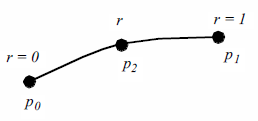
\includegraphics[width=\linewidth]{Figure8-16}
            \caption*{}
        \end{subfigure}
        \hfill
        \begin{subfigure}{0.48\linewidth}
            \centering
            \begin{equation*}
            \begin{array}{lll}
            W_0 &=& 2 \left( r - \dfrac{1}{2}\right)(r - 1) \\ \\
            W_1 &=& 2 r \left( r - \dfrac{1}{2}\right) \\ \\
            W_2 &=& 4 r (1 - r)
            \end{array}
            \end{equation*}
        \end{subfigure}%
        \caption{Parametric coordinate system and interpolation functions for a quadratic wedge.}
        \label{fig:Figure8-16}
    \end{figure}

    \item[Tetrahedron.] Figure \ref{fig:Figure8-9} shows the parametric coordinate system and interpolation functions for a tetrahedron cell type. The tetrahedron is described using the three parametric coordinates $(r,s,t)$.

    \item[Voxel.] Figure \ref{fig:Figure8-10} shows the parametric coordinate system and interpolation functions for a voxel cell type. The voxel is described using the three parametric coordinates $(r,s,t)$. Note that the voxel edges are constrained to lie parallel to the global coordinate axes. These are often referred to as \emph{trilinear interpolation} functions.

%\clearpage
    \begin{figure}[!htb]
        \centering
        \begin{subfigure}{0.48\linewidth}
            \centering
            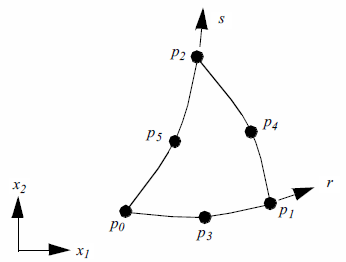
\includegraphics[width=\linewidth]{Figure8-17}
            \caption*{}
        \end{subfigure}
        \hfill
        \begin{subfigure}{0.48\linewidth}
            \centering
            \begin{equation*}
            \begin{array}{lll}
            W_0 &=& (1 - r - s)(2(1 - r - s) - 1) \\
            W_1 &=& r (2 r - 1) \\
            W_2 &=& s(2s - 1) \\
            W_3 &=& 4 r (1 - r - s) \\
            W_4 &=& 4 r s \\
            W_5 &=& 4 s (1 - r - s)
            \end{array}
            \end{equation*}
        \end{subfigure}%
        \caption{Parametric coordinate system and interpolation functions for a quadratic triangle.}
        \label{fig:Figure8-17}
    \end{figure}

    \begin{figure}[!htb]
        \centering
        \begin{subfigure}{0.48\linewidth}
            \centering
            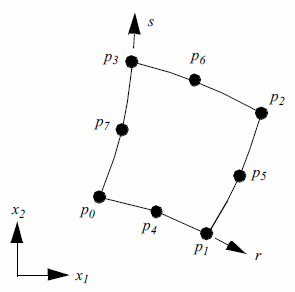
\includegraphics[width=\linewidth]{Figure8-18}
            \caption*{}
        \end{subfigure}
        \hfill
        \begin{subfigure}{0.48\linewidth}
            \centering
            \begin{equation*}
            \begin{array}{lll}
            \xi &=& 2 r  - 1, \quad \xi_i = \pm 1 \\
            \eta &=& 2 s - 1, \quad \eta_i = \pm 1
            \end{array}
            \end{equation*}
            \begin{equation*}
            \begin{array}{lll}
            W_i &=& (1 + \xi_i \xi)(1 + \eta_i \eta)(\xi_i \xi + \eta_i \eta - 1)/4, \\
            i &\in& \lbrace 0, 1, 2, 3, 4 \rbrace \\ \\
            W_i &=& (1 - \xi^2)(1 + \eta_i \eta)/2,\\
            i &\in& \lbrace 4, 6 \rbrace  \\ \\
            W_i &=& (1 - \eta^2)(1 + \xi_i \xi)/2, \\
            i &\in& \lbrace 5, 7 \rbrace
            \end{array}
            \end{equation*}
        \end{subfigure}%
        \caption{Parametric coordinate system and interpolation functions for a quadratic quadrilateral. In VTK parametric coordinates $(r,s)$ run between (0,1), hence the coordinate system shift into the $(\xi, \eta$) parametric system ranging from $(-1,1)$. Note that $\xi_i$ and $\eta_i$ refer to the parametric coordinates of the $i^{th}$ point.}
        \label{fig:Figure8-18}
    \end{figure}

    \item[Hexahedron.] Figure \ref{fig:Figure8-11} shows the parametric coordinate system and interpolation functions for a hexahedron cell type. The hexahedron is described using the three parametric coordinates $(r,s,t)$.

    \item[Wedge.] Figure \ref{fig:Figure8-12} shows the parametric coordinate system and interpolation functions for a wedge cell type. The wedge is described using the three parametric coordinates $(r,s,t)$.

    \item[Pyramid.] Figure \ref{fig:Figure8-13} shows the parametric coordinate system and interpolation functions for a pyramid cell type. The pyramid is described using the three parametric coordinates $(r,s,t)$.

    \item[Pentagonal Prism.] Figure \ref{fig:Figure8-14} shows the parametric coordinate system and interpolation functions for a pentagonal prism cell type. The pentagonal prism is described using the three parametric coordinates $(r,s,t)$.

%\clearpage
    \begin{figure}[!htb]
        \centering
        \begin{subfigure}{0.48\linewidth}
            \centering
            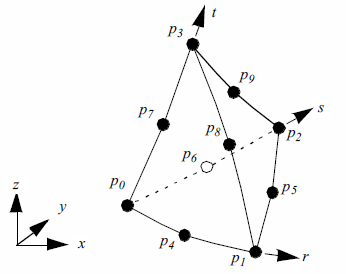
\includegraphics[width=\linewidth]{Figure8-19}
            \caption*{}
        \end{subfigure}
        \hfill
        \begin{subfigure}{0.48\linewidth}
            \centering
            \begin{equation*}
            \begin{array}{lll}
            u &=& 1 - r - s- t \\ \\
            W_0 &=& u(2u-1) \\
            W_1 &=& r(2r - 1) \\
            W_2 &=& s(2s - 1) \\
            W_3 &=& t (2t - 1)
            \end{array}
            \end{equation*}
            \noindent\begin{minipage}{.5\linewidth}
                \begin{equation*}
                \begin{array}{lll}
                W_4 &=& 4 u r \\
                W_5 &=& 4 r s \\
                W_6 &=& 4 s u
                \end{array}
                \end{equation*}
            \end{minipage}%
            \noindent\begin{minipage}{.5\linewidth}
                \begin{equation*}
                \begin{array}{lll}
                W_7 &=& 4 u t \\
                W_8 &=& 4 r t \\
                W_9 &=& 4 s t
                \end{array}
                \end{equation*}
            \end{minipage}%

        \end{subfigure}%
        \caption{Parametric coordinate system and interpolation functions for a quadratic tetrahedron. In VTK parametric coordinates $(r,s,t)$ run between $(0,1)$, hence the coordinate system shift into the $(\xi, \eta, \zeta)$ parametric system ranging from $(-1,1)$.}
        \label{fig:Figure8-19}
    \end{figure}

    \begin{figure}[!htb]
        \centering
        \begin{subfigure}{0.48\linewidth}
            \centering
            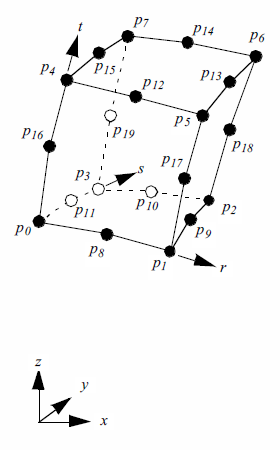
\includegraphics[width=\linewidth]{Figure8-20}
            \caption*{}
        \end{subfigure}
        \hfill
        \begin{subfigure}{0.48\linewidth}
            \begin{equation*}
            \begin{array}{lll}
            \xi &=& 2r  - 1,\quad \xi_i = \pm1 \\
            \eta &=& 2 s - 1,\quad \eta_i = \pm1 \\
            \zeta &=& 2 t - 1,\quad \zeta_i = \pm1
            \end{array}
            \end{equation*}
            \begin{equation*}
            \begin{array}{lll}
            W_i &=& (1 + \xi_i \xi)(1 + \eta_i \eta)(1 + \zeta_i \zeta)(\xi_i \xi + \eta_i \eta + \zeta_i \zeta - 2)/8, \\
            i &\in& \lbrace 1 \ldots 7 \rbrace \\ \\
            W_i &=& (1 - \xi^2)(1 + \eta_i \eta)(1 + \zeta_i \zeta)/4, \\
            i &\in& \lbrace 8, 10, 12, 14 \rbrace \\ \\
            W_i &=& (1 - \eta^2)(1 + \xi_i \xi)(1 + \zeta_i \zeta)/4, \\
            i &\in& \lbrace 9, 11, 13, 15 \rbrace \\ \\
            W_i &=& (1 - \zeta^2)(1 + \xi_i \xi)(1 + \eta_i \eta)/4, \\
            i &\in& \lbrace 16, 17, 18, 19 \rbrace
            \end{array}
            \end{equation*}
        \end{subfigure}%
        \caption{Parametric coordinate system and interpolation functions for a quadratic hexahedron. In VTK parametric coordinates $(r,s,t)$ run between $(0,1)$, hence the coordinate system shift into the $(\xi, \eta, \zeta)$ parametric system ranging from (-1,1). Note that $\xi_i$, $\eta_i$ and $\zeta_i$ refer to the parametric coordinates of the $i^{th}$ point.}
        \label{fig:Figure8-20}
    \end{figure}

    \begin{figure}[!htb]
        \centering
        \begin{subfigure}{0.48\linewidth}
            \centering
            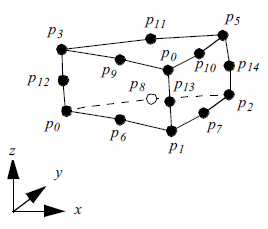
\includegraphics[width=\linewidth]{Figure8-21}
            \caption*{}
        \end{subfigure}
        \hfill
        \begin{subfigure}{0.48\linewidth}
            \centering
            \begin{equation*}
            \begin{array}{lll}
            W_0 &=& (1 - r - s)(1 - t)(1 - 2r -2s -2t) \\
            W_1 &=& r(1 - t)(2r - 2t - 1) \\
            W_2 &=& s(1 - t)(2s - 2t - 1) \\
            W_3 &=& (1 - r - s)t(2t - 2r - 2s - 1) \\
            W_4 &=& rt(2r + 2t - 3) \\
            W_5 &=& st(2s + 2t - 3) \\
            W_6 &=& 4r(1 - r - s)(1 - t) \\
            W_7 &=& 4rs(1 - t) \\
            W_8 &=& 4s(1 - t)(1 - r - s) \\
            W_9 &=& 4r(1 - r - s)t \\
            W_{10} &=& 4 rst \\
            W_{11} &=& 4 (1 - r - s)s t\\
            W_{12} &=& 4 (1 - r - s)t(1 - t) \\
            W_{13} &=& 4rt(1 - t) \\
            W_{14} &=& 4st(1 - t)
            \end{array}
            \end{equation*}
        \end{subfigure}%
        \caption{Parametric coordinate system and interpolation functions for a quadratic wedge.}
        \label{fig:Figure8-21}
    \end{figure}

    \item[Hexagonal Prism.] Figure \ref{fig:Figure8-15} shows the parametric coordinate system and interpolation functions for a hexagonal prism cell type. The hexagonal prism is described using the three parametric coordinates $(r,s,t)$.

    \item[Quadratic Edge.] Figure \ref{fig:Figure8-16} shows the parametric coordinate system and interpolation functions for a quadratic edge cell type. The quadratic edge is described using the single parametric coordinate $r$.

    \item[Quadratic Triangle.] Figure \ref{fig:Figure8-17} shows the parametric coordinate system and interpolation functions for a quadratic triangle cell type. The quadratic triangle is described using the two parametric coordinates $(r,s)$.

    \item[Quadratic Quadrilateral.] Figure \ref{fig:Figure8-18} shows the parametric coordinate system and interpolation functions for a quadratic quadrilateral cell type. The quadratic quadrilateral is described using the two parametric coordinates $(r,s)$. Note that because the interpolation functions are most easily expressed in the interval $(-1,1)$, a coordinate shift is performed to the $(\xi, \eta)$ coordinates defined in this range. Also, the notation $\xi_i$ and $\eta_i$ is introduced. These are the parametric coordinates at the $i^{th}$ point.

%\clearpage
    \begin{figure}[!htb]
        \centering
        \begin{subfigure}{0.48\linewidth}
            \centering
            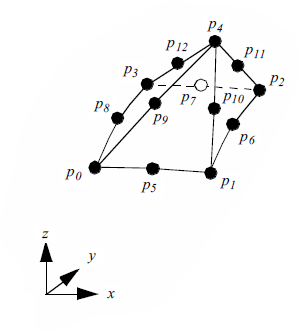
\includegraphics[width=\linewidth]{Figure8-22}
            \caption*{}
        \end{subfigure}
        \hfill
        \begin{subfigure}{0.48\linewidth}
            \centering
            \begin{equation*}
            \begin{array}{lll}
            \xi &=& 2 r - 1, \quad \xi_i = \pm1 \\ \\
            \eta &=& 2 s - 1, \quad \eta_i = \pm1 \\ \\
            \zeta &=& 2 t - 1, \quad \zeta_i = \pm1
            \end{array}
            \end{equation*}
            \begin{equation*}
            \begin{array}{lll}
            W_i &=& (1 + \xi_i \xi)(1 + \eta_i \eta)(1 + \zeta_i \zeta)(\xi_i \xi + \eta_i \eta + \zeta_i \zeta - 2)/8, \\
            i &\in& \lbrace 0, 1, 2, 3 \rbrace \\
            W_4 &=& \zeta(1 - \zeta)/4, \quad i \in \lbrace 4 \rbrace \\
            W_i &=& (1 - \xi^2)(1 + \eta_i \eta)(1 + \zeta_i \zeta)/4, \quad i \in \lbrace 5, 6, 7, 8\rbrace \\
            W_i &=& (1 - \zeta^2)(1 + \xi_i \xi)(1 + \eta_i \eta)/4, \quad i \in \lbrace 9, 10, 11, 12 \rbrace
            \end{array}
            \end{equation*}
        \end{subfigure}%
        \caption{Parametric coordinate system and interpolation functions for a quadratic pyramid. In VTK parametric coordinates $(r,s,t)$ run between $(0,1)$, hence the coordinate system shift into the $(\xi, \eta, \zeta)$ parametric system ranging from (-1,1). Note that $\xi_i$, $\eta_i$ and $\zeta_i$ refer to the parametric coordinates of the $i^{th}$ point.}
        \label{fig:Figure8-22}
    \end{figure}

    \item[Quadratic Tetrahedron.] Figure \ref{fig:Figure8-19} shows the parametric coordinate system and interpolation functions for a quadratic tetrahedron cell type. The quadratic tetrahedron is described using the three parametric coordinates $(r,s,t)$.

    \item[Quadratic Hexahedron.] Figure \ref{fig:Figure8-20} shows the parametric coordinate system and interpolation functions for a quadratic hexahedron cell type. The quadratic hexahedron is described using the three parametric coordinates $(r,s,t)$. Note that because the interpolation functions are most easily expressed in the interval $(-1,1)$, a coordinate shift is performed to the $(\epsilon, \eta, \zeta)$ coordinates defined in this range. Also, the notation $\epsilon_i$, $\eta_i$ and $\zeta_i$ is introduced. These are the parametric coordinates at the $i{th}$ point.

    \item[Quadratic Wedge.] Figure \ref{fig:Figure8-21} shows the parametric coordinate system and interpolation functions for a quadratic wedge cell type. The quadratic wedge is described using the three parametric coordinate $(r,s,t)$.

    \item[Quadratic Pyramid.] Figure \ref{fig:Figure8-22} shows the parametric coordinate system and interpolation functions for a quadratic pyramid cell type. The quadratic pyramid is described using the three parametric coordinates $(r,s,t)$. Note that because the interpolation functions are most easily expressed in the interval $(-1,1)$, a coordinate shift is performed to the $(\epsilon, \eta, \zeta)$ coordinates system defined in this range. Also, the notation $\epsilon_i$, $\eta_i$ and $\zeta_i$ is introduced, these are the parametric coordinate at the $i^{th}$ point. (The shape functions and derivatives were implemented thanks to the \href{https://www.colorado.edu/aerospacestructures/}{Center For Aerospace Structures}.)  
 
\end{description}
\index{interpolation function|)}

\section{Cell Tessellation}

\begin{wrapfigure}{R}{0.4\textwidth}
	\centering
	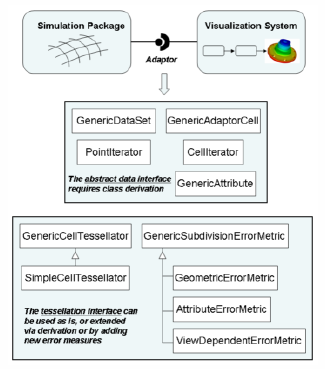
\includegraphics[width=0.98\textwidth]{Figure8-23}
	\caption{Cell adaptor framework.}
	\label{fig:Figure8-23}
\end{wrapfigure}

As briefly introduced in Chapter 5: \nameref{chap:basic_data_representation}, nonlinear cells are often used in various numerical techniques such as the finite element method. While some visualizatinon systems support nonlinear cells directly, typically only quadratic and occasionally cubic formulations are supported (for example, VTK supports quadratic cells). This represents only a small subset of the formulations currently available in numerical packages, and ignores the unlimited potential cell formulations. To address this important problem, visualization systems may provide an adaptor framework\index{cell!adaptor framework} (see Figure \ref{fig:Figure8-23}) that enables users to interface their own simulation system to the visualization system \cite{Schroeder06}. Such a framework requires writing adaptor classes that are derived from visualization dataset and cell base classes (in the figure these are labeled GenericDataSet\index{GenericDataSet} and GenericAdaptorCell\index{GenericAdaptorCell}). These adaptors act like translators, converting data and method invocations to and from the forms expected by the visualization system and the numerical system. Like any other data objects, such adaptor cells and datasets can be processed directly by visualization algorithms. However, processing such general data objects is a difficult problem, since most visualization algorithms described in the scientific literature to date adopt the fundamental assumptions that cell geometry is linear. Removing this assumption may require introducing significant complexity into the algorithm, or may even require a new algorithm. For example, the marching cubes isocontouring algorithm assumes that the cells are ortho--rectilinear hexahedra; without this assumption elaborate transformations to and from parametric and global coordinate systems are required, and even then in highly curved nonlinear cells, degenerate or self-intersection isocontours may be generated without extensive topological and geometric checks. Thus the adaptor framework typically includes methods for tessellating nonlinear cells into the familiar linear cells, which can then be readily processed by conventional visualization algorithms. In the following section, we briefly described a simple method for tessellating higher order, nonlinear cells to produce linear cells.

\subsection{Basic Approach}

The basic approach is to dynamically tessellate the cells of the GenericDataSet\index{GenericDataSet}, and then operate on the resulting linear tessellation. As expressed in pseudo-code, a typical algorithm looks like this:

\begin{lstlisting}[caption={}, numbers=none, frame=none]
for each cell c to be processed
  {
  if cell c meets selection criteria
    {
    linearDataSet = TessellateCell(c)
    for each linear cell cl in linearDataSet
      {
      OperateOn(cl)
      }
    }
 }
\end{lstlisting}

It is important not to tessellate the entire dataset all at once, since this may produce excessive demands on memory resources, and many algorithms visit only a subset of a dataset's cells. Thus the pseudo-code above refers to a selection criterion, which varies depending on the nature of the algorithm. For example, an isocontouring algorithm may check to see whether the cell's scalar values span the current isocontour value.

While many tessellation algorithms are possible, those based on edge subdivision are particularly simple. The idea behind the algorithm is simple: each cell edge $e$ is evaluated via an error metric $E$ and may be marked for subdivision if any error measure $\epsilon_i$ exceeds a corresponding error threshold $\epsilon_i^T$  

\begin{equation}\label{eq:8.7}
\text{split edge if} (\epsilon_i > \epsilon_i^{\text{T}}), \quad \text{for any} \quad \epsilon_i \in E
\end{equation}
\myequations{Condition for splitting an edge.}

Based on the cell topology, and the particular edges requiring subdivision, templates are used to subdivide the cell. This process continues recursively until the error metric is satisfied on all edges. One advantage of this algorithm is that cells can be tessellated independently. This is because edge subdivision is a function of one or more error measures that consider only information along the edge, and does not need to take into account cell information. Therefore no communication across cell boundaries is required, and the algorithm is well suited for parallel processing and on the fly tessellation as cells are visited during traversal.

\begin{figure}[!htb]
    \centering
    \begin{subfigure}{0.32\linewidth}
        \centering
        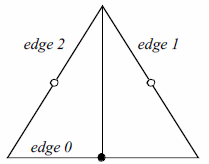
\includegraphics[width=\linewidth]{Figure8-24a}
        \caption{Case 001}\label{fig:Figure8-24a}
    \end{subfigure}
    \hfill
    \begin{subfigure}{0.32\linewidth}
        \centering
        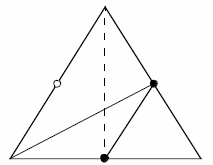
\includegraphics[width=\linewidth]{Figure8-24b}
        \caption{Case 011}\label{fig:Figure8-24b}
    \end{subfigure}%
    \hfill
    \begin{subfigure}{0.32\linewidth}
        \centering
        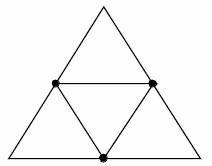
\includegraphics[width=\linewidth]{Figure8-24c}
        \caption{Case 111}\label{fig:Figure8-24c}
    \end{subfigure}%
    \caption{Three cases from the subdivision table for a triangle. Filled circles indicate that the edge is marked for subdivision.}
    \label{fig:Figure8-24}
\end{figure}

Some templates for cell subdivision are shown in Figure \ref{fig:Figure8-24}. Note that in some cases a choice must be made in terms of which diagonal to select for tessellation (for example, the dashed line in Figure ref{fig:Figure8-24b}). In 2D, this choice can be made arbitrarily, however in 3D the choice must be consistent with the cell's face neighbor. In order to preserve the simplicity of the algorithm, including avoiding inter-cell communication, simple tie-breaking rules for selecting the diagonal on the faces of 3D cells are adopted. These rules include using the shortest diagonal (measured in the global coordinate system), or using a topological decider based on selecting the diagonal with the smallest point id. (A topological decider is necessary when the geometric distance measure is inconclusive.)

\subsection{Error Measures}

The algorithm described above is adaptive because edge splitting is controlled by local mesh properties and/or its relation to the view position. Since the goal is to insure that the quality of the tessellation is consistent with the particular requirements of the visualization, we expect the adapted tessellation to be of better quality as compared to a fixed subdivision with the same number of simplices, or have fewer simplices for tessellations of equal quality.

\begin{wrapfigure}{R}{0.4\textwidth}
	\centering
	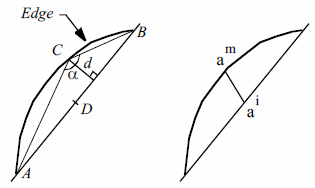
\includegraphics[width=0.98\textwidth]{Figure8-25}
	\caption{Cell adaptor framework.}
	\label{fig:Figure8-25}
\end{wrapfigure}

Our design allows for the definition of multiple error measures. As indicated in Equation 8-7, the error metric consists of several error measures, each of which evaluates local properties of the edge against the linear approximation, and compares the measure against a user-specified threshold. If any measure exceeds the threshold, then the edge is subdivided. These error measures may evaluate geometric properties, approximation to solution attributes, or error related to the current view, among other possibilities. Error measures based on geometry or attributes are independent of view and the mesh requires only one initial tessellation.

The following paragraphs describes several error measures that have been found to be useful in practice. Since the tessellator is designed to process a list of error measures, it is straightforward to add new ones (by deriving from the GenericSubdivisionErrorMetric\index{GenericSubdivisionErrorMetric} class) and/or combine it with existing error measures.
\begin{description}

    \item [\textit{Object-Based Geometric Error Measure.}] Referring to Figure \ref{fig:Figure8-25}(left), this error measure is the perpendicular distance, $d$, from the edge center point $C$ to the straight line passing through the cell edge vertices ($A$ and $B$). Note that $d$ is computed in world coordinates, but $C$ is computed by evaluation at the parametric center of the edge. The perpendicular distance is used rather than the distance between $C$ and $D$ because if $C$ lies on $(AB)$ but is not coincident with $D$ the error is non-zero, resulting in many useless edge subdivisions.

    \item [\textit{Object-Based Flatness Error Measure.}] This error measure is the angle $\alpha$ between the chords $(AC)$ and $(CB)$ passing through the real mid-point $C$. As the angle approaches $180\deg$ the edge becomes flat. The threshold is the angle over which the edge is viewed as flat.

    \item [\textit{Attribute-Based Error Measure.}] Referring to Figure \ref{fig:Figure8-25}(right), this error measure is the distance between ai the linearly interpolated value of an attribute at the midpoint and the actual value of this attribute at the edge midpoint $a^m$.

    \item [\textit{Image-Based Geometric Error Measure.}] This error measure is the distance, in pixels, between the line $(AB)$ projected in image space to the midpoint $C$ also projected in image space. Because the computation involves projection through the current camera matrix, this error measure is view-dependent. As a result, the tessellation may be crude in portions of the mesh away from the camera. Note that one of the disadvantages of this approach is that tessellation may be required each time the camera is repositioned relative to the mesh.

\end{description}

\subsection{Advanced Methods}

Attentive readers will have noticed that the subdivision scheme described previously may fail to capture all the features of the higher-order basis. For example, imagine a scalar function across a triangle where the peak value of the function occurs in the center of the triangle, and the variation across the edges is zero. The edge subdivision algorithm described previously will not capture the peak, hence an algorithm such as isocontouring will produce inaccurate results. Linear isocontouring algorithms require that the following conditions are met in order to produce topologically correct results.

\begin{itemize}

\item each mesh edge intersects an isocontour of a particular value at most once,

\item intersects a mesh face without intersecting at least two edges of the face, and

\item is completely contained within a single element.

\end{itemize}

By definition, these conditions are directly related to critical points, since an extremum of a differentiable function over an open domain is necessarily a critical point. Linear meshes assume that all extrema of the scalar field occur at element vertices, but in general when using a higher-order basis this is not the case, and extrema can be found interior to a cell.

To address this problem, a pre-triangulation of the basis must be performed. The pre--triangulation must identify all critical points in the interior, on the faces, or on the edge of a cell, and then insert these points into the triangulation. For example, an initial triangulation based on the vertices of the higher-order cell can be performed first, followed by insertion into the triangulation using a method such as Delaunay triangulation or equivalent (see ``Triangulation'' on page \pageref{subsec:decimation.triangulation}). The pre--triangulation can then be followed by the standard edge--based algorithm presented previously.

\section{Coordinate Transformation}
\index{coordinate transformation|(}

Coordinate transformation is a common visualization operation. This may be either transformation from dataset coordinates to global coordinates, or global coordinates to dataset coordinates.

\subsection{Dataset to Global Coordinates}
\index{coordinate transformation!dataset to global|(}

Transforming between dataset coordinates and global coordinates is straightforward. We start by identifying a primary cell using the cell id and sub-id. Then the global coordinates are generated from the parametric coordinates by using the interpolation functions of Equation \ref{eq:8.4}. Given cell points $p_i = p_i(x_i, y_i, z_i)$ the global coordinate $p$ is simply

\begin{equation}\label{eq:8.8}
p = \sum_{i = 0}^{n - 1} W_i(r_0, s_0, t_0)\, p_i
\end{equation}
\myequations{Generating global coordinates from parametric ones.}

where the interpolation weights $W_i$i are evaluated at the parametric coordinate $(r_0, s_0, t_0)$.

In the formulation presented here, we have used the same order interpolation functions for both data and cell geometry. (By order we mean the polynomial degree of the interpolating polynomials.) This is termed iso--parametric interpolation. It is possible to use different interpolation functions for geometry and data. Super--parametric interpolation is used when the order of the interpolation functions for geometry is greater than those used for data. Sub-parametric interpolation is used when the order of the interpolation functions for geometry is less than those used for data. Using different interpolation functions is commonly used in numerical analysis techniques such as the finite element method. We will always use the iso--parametric interpolation for visualization applications.
\index{coordinate transformation!dataset to global|)}

\subsection{Global to Dataset Coordinates}
\index{coordinate transformation!global to dataset|(}

Global to dataset coordinate transformations are expensive compared to dataset to global transformations. There are two reasons for this. First, we must identify the particular cell $C_i$ that contains the global point p. Second, we must solve Equation \ref{eq:8.4} for the parametric coordinates of $p$.

To identify the cell $C_i$ means doing some form of searching. A simple but inefficient approach is to visit every cell in a dataset and determine whether p lies inside any cell. If so, then we have found the correct cell and stop the search. Otherwise, we check the next cell in the list.

This simple technique is not fast enough for large data. Instead, we use accelerated search techniques. These are based on spatially organizing structures such as an octree or three-dimensional hash table. The idea is as follows: we create a number of ``buckets'', or data place holders, that are accessed by their location in global space. Inside each bucket we tag all the points or cells that are partially or completely inside the bucket. Then, to find a particular cell that contains point $p$, we find the bucket that contains $p$, and obtain all the cells associated with the bucket. We then evaluate inside/outside for this abbreviated cell list to find the single cell containing p. (See ``Searching'' on page \pageref{sec:searching} for a more detailed description.)

The second reason that global to dataset coordinate transformation is expensive is because we must solve the interpolation function for the parametric coordinates of p. Sometimes we can do this analytically, but in other cases we must solve for the parametric coordinates using numerical techniques.

Consider the interpolation functions for a line (Figure \ref{fig:Figure8-2}). We can solve this equation exactly and find that

\begin{equation}\label{eq:8.9}
r = \frac{x - x_0}{x_1 - x_0} = \frac{y - y_0}{y_1 - y_0} = \frac{z - z_0}{z_1 - z_0}
\end{equation}
\myequations{Interpolation functions for a line.}

Similar relations exist for any cell whose interpolation functions are linear combinations of parametric coordinates. This includes vertices, lines, triangles, and tetrahedra. The quadrilateral and hexahedron interpolation functions are nonlinear because they are products of linear expressions for the parametric coordinates. As a result, we must resort to numerical techniques to compute global to dataset coordinate transformations. The interpolation functions for pixels and voxels are nonlinear as well, but because of their special orientation with respect to the $x$, $y$, and $z$ coordinate axes, we can solve them exactly. (We will treat pixel and voxel types in greater depth in ``Special Techniques for Image Data'' on page \pageref{sec:special_techniques_for_image_data}.)

To solve the interpolation functions for parametric coordinates we must use nonlinear techniques for the solution of a system of equations. A simple and effective technique is Newton's method \cite{Conte72}.

To use Newton's method we begin by defining three functions for the known global coordinate $p = p(x,y,z)$ in terms of the interpolation functions $W_i = W_i(r,s,t)$

\begin{equation}\label{eq:8.10}
\begin{array}{lll}
f(r, s, t) &=& x - \sum W_i \, x_i = 0 \\ \\
g(r, s, t) &=& y - \sum W_i \, y_i = 0 \\ \\
h(r, s, t) &=& z - \sum W_i \, z_i = 0
\end{array}
\end{equation}
\myequations{Global coordinates in terms of interpolation functions.}

and then, expanding the functions using a Taylor's series approximation,

\begin{equation}\label{eq:8.11}
\begin{array}{lll}
f(r, s, t) &\simeq& f_0
  + \dfrac{\partial f}{\partial r}(r - r_0)
  + \dfrac{\partial f}{\partial s}(s - s_0)
  + \dfrac{\partial f}{\partial t}(t - t_0) + \ldots \\ \\
g(r, s, t) &\simeq& g_0
  + \dfrac{\partial g}{\partial r}(r - r_0)
  + \dfrac{\partial g}{\partial s}(s - s_0)
  + \dfrac{\partial g}{\partial t}(t - t_0) + \ldots \\ \\
h(r, s, t) &\simeq& h_0
  + \dfrac{\partial h}{\partial r}(r - r_0)
  + \dfrac{\partial h}{\partial s}(s - s_0)
  + \dfrac{\partial h}{\partial t}(t - t_0) + \ldots
\end{array}
\end{equation}
\myequations{Taylor series approximations of global coordinates in terms of interpolation functions.}

\begin{equation}\label{eq:8.12}
\left(
\begin{array}{c}
r_{i + 1} \\ \\
s_{i + 1} \\ \\
t_{i + 1}
\end{array}
\right) = \left(
\begin{array}{c}
r_i \\ \\
s_i \\ \\
t_i
\end{array}
\right) - \left(
\begin{array}{c c c}
\dfrac{\partial f}{\partial r} & \dfrac{\partial f}{\partial s} & \dfrac{\partial f}{\partial t} \\ \\
\dfrac{\partial g}{\partial r} & \dfrac{\partial g}{\partial s} & \dfrac{\partial g}{\partial t} \\ \\
\dfrac{\partial h}{\partial r} & \dfrac{\partial h}{\partial s} & \dfrac{\partial h}{\partial t}
\end{array}
\right)^{-1}
\left(
\begin{array}{c}
f_i \\ \\
g_i \\ \\
h_i
\end{array}
\right)
\end{equation}
\myequations{Using iteration to solve for the parametric coordinates.}

Fortunately, Newton's method converges quadratically (if it converges) and the interpolation functions that we have presented here are well behaved. In practice, Equation \ref{eq:8.12} converges in just a few iterations.
\index{coordinate transformation!global to dataset|)}
\index{coordinate transformation|)}

\section{Computing Derivatives}
\index{derivatives|(}

\begin{figure}[!htb]
    \centering
    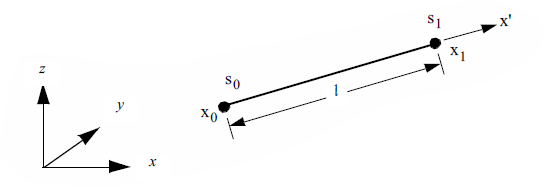
\includegraphics[width=0.98\textwidth]{Figure8-26}\\
    \caption{Computing derivatives in an 1D line cell.}\label{fig:Figure8-26}
\end{figure}

Interpolation functions enable us to compute data values at arbitrary locations within a cell. They also allow us to compute the rate of change, or derivatives, of data values. For example, given displacements at cell points we can compute cell strains and stresses --- or, given pressure values, we can compute the pressure gradient at a specified location.

To introduce this process, we will begin by examining the simplest case: computing derivatives in a 1D line (Figure \ref{fig:Figure8-26}). Using geometric arguments, we can compute the derivatives in the r parametric space according to

\begin{equation}\label{eq:8.13}
\dfrac{d s}{d r} = \dfrac{s_1 - s_0}{1} = (s_1 - s_0)
\end{equation}
\myequations{Computing derivatives in a parametric space.}

where $s_i$ is the data value at point $i$. In the local coordinate system $x'$, which is parallel to the $r$ coordinate system (that is, it lies along the vector $\overrightarrow{x_1} - \overrightarrow{x_0})$, the derivative is

\begin{equation}\label{eq:8.14}
\dfrac{d s}{d x'} = \dfrac{s_1 - s_0}{1}
\end{equation}
\myequations{The derivative in a local coordinate space.}

where $l$ is the length of the line.

Another way to derive Equation \ref{eq:8.14} is to use the interpolation functions of Figure \ref{fig:Figure8-3} and the chain rule for derivatives. The chain rule

\begin{equation}\label{eq:8.15}
\dfrac{d}{d r} = \dfrac{d}{dx'} \dfrac{dx'}{dr}
\end{equation}
\myequations{The chain rule for derivatives.}

allows us to compute the derivative $\dfrac{d}{dx'}$ using

\begin{equation}\label{eq:8.16}
\frac{d}{d x'} = \dfrac{d}{dr}/ \dfrac{dx'}{dr}
\end{equation}
\myequations{Computing the derivative $\dfrac{d}{dx'}$.}

With the interpolation functions we can compute the $x'$ derivatives with respect to $r$ as

\begin{equation}\label{eq:8.17}
\frac{d x'}{d r} = \frac{d}{dr} \left(\sum_{i}W_i \, x_i' \right) = -x_0' + x_1' = 1
\end{equation}
\myequations{Computing the $x'$ derivatives with respect to $r$.}

which, when combined with Equation \ref{eq:8.16} and Equation \ref{eq:8.13} for the $s$ derivatives, yields Equation \ref{eq:8.14}.

One final step remains. The derivatives in the $\overrightarrow{x\ }$ coordinate system must be converted to the global $x-y-z$ system. We can do this by creating a unit vector $\overrightarrow{v}$ as

\begin{equation}\label{eq:8.18}
\overrightarrow{v\ } = \frac{\overrightarrow{x_1} - \overrightarrow{x_0 }}{\vert\overrightarrow{x_1} - \overrightarrow{x_0} \vert}
\end{equation}
\myequations{Creating the unit vector.}

where $\overrightarrow{x_0}$ and $\overrightarrow{x_1}$ are the locations of the two end points of the line. Then the derivatives in the $x$, $y$, and $z$ directions can be computed by taking the dot products along the axes.

\begin{equation}\label{eq:8.19}
\begin{array}{lll}
\dfrac{ds}{dx}  &=& \left(\dfrac{s_1 - s_0}{1}\right) \overrightarrow{v\ } \cdot (1, 0, 0) \\ \\
\dfrac{ds}{dy}  &=& \left(\dfrac{s_1 - s_0}{1}\right) \overrightarrow{v\ } \cdot (0, 1, 0) \\ \\
\dfrac{ds}{dz}  &=& \left(\dfrac{s_1 - s_0}{1}\right) \overrightarrow{v\ } \cdot (0, 0, 1)
\end{array}
\end{equation}
\myequations{Derivatives in the $x$, $y$, and $z$ directions.}

To summarize this process, derivatives are computed in the local $r-s-t$ parametric space using cell interpolation. These are then transformed into a local $x'-y'-z'$ Cartesian system. Then, if the $x'-y'-z'$ system is not aligned with the global $x-y-z$ coordinate system, another transformation is required to generate the result.

We can generalize this process to three dimensions. From the chain rule for partial derivatives

\begin{equation}\label{eq:8.20}
\begin{array}{lll}
\dfrac{\partial}{\partial x} &=& \dfrac{\partial}{\partial r} \dfrac{\partial r}{\partial x} \
+ \dfrac{\partial}{\partial s} \dfrac{\partial s}{\partial x} \
+ \dfrac{\partial}{\partial t} \dfrac{\partial t}{\partial x} \\ \\
\dfrac{\partial}{\partial y} &=& \dfrac{\partial}{\partial r} \dfrac{\partial r}{\partial y} \
+ \dfrac{\partial}{\partial s} \dfrac{\partial s}{\partial y} \
+ \dfrac{\partial}{\partial t} \dfrac{\partial t}{\partial y} \\ \\
\dfrac{\partial}{\partial z} &=& \dfrac{\partial}{\partial r} \dfrac{\partial r}{\partial z} \
+ \dfrac{\partial}{\partial s} \dfrac{\partial s}{\partial z} \
+ \dfrac{\partial}{\partial t} \dfrac{\partial t}{\partial z}
\end{array}
\end{equation}
\myequations{Chain rule for partial derivatives.}

or after rearranging

\begin{equation}\label{eq:8.21}
\begin{array}{lll}
\left(
\begin{array}{c}
\dfrac{\partial}{\partial r} \\ \\
\dfrac{\partial}{\partial s} \\ \\
\dfrac{\partial}{\partial t}
\end{array}
\right) = \left(
\begin{array}{c c c}
\dfrac{\partial x}{\partial r} & \dfrac{\partial y}{\partial r} & \dfrac{\partial z}{\partial r} \\ \\
\dfrac{\partial x}{\partial s} & \dfrac{\partial y}{\partial s} & \dfrac{\partial z}{\partial s} \\ \\
\dfrac{\partial x}{\partial t} & \dfrac{\partial y}{\partial t} & \dfrac{\partial z}{\partial t}
\end{array}
\right)
\left(
\begin{array}{c}
\dfrac{\partial}{\partial x} \\ \\
\dfrac{\partial}{\partial y} \\ \\
\dfrac{\partial}{\partial z}
\end{array}
\right) =
\mathbf{J}\left(
\begin{array}{c}
\dfrac{\partial}{\partial x} \\ \\
\dfrac{\partial}{\partial y} \\ \\
\dfrac{\partial}{\partial z}
\end{array}
\right)
\end{array}
\end{equation}
\myequations{Chain rule for partial derivatives (rearranged).}

The $3 \times 3$ matrix $\mathbf{J}$ is called the Jacobian matrix, and it relates the parametric coordinate derivatives to the global coordinate derivatives. We can rewrite Equation \ref{eq:8.21} into more compact form

\begin{equation}\label{eq:8.22}
\dfrac{\partial}{\partial r_i} = \sum_{j} \mathbf{J}_{ij} \dfrac{\partial}{\partial x_j}
\end{equation}
\myequations{Jacobian form of partial derivatives.}

and solve for the global derivatives by taking the inverse of the Jacobian matrix

\begin{equation}\label{eq:8.23}
\frac{\partial}{\partial x_i} = \sum_{j} \mathbf{J}_{ij}^{-1} \frac{\partial}{\partial r_j}
\end{equation}
\myequations{Inverse Jacobian form of partial derivatives.}

The inverse of the Jacobian always exists as long as there is a one--to--one correspondence between the parametric and global coordinate systems. This means that for any $(r, s, t)$ coordinate, there corresponds only one $(x, y, z)$ coordinate. This holds true for any of the parametric coordinate systems presented here, as long as pathological conditions such as cell self--intersection or a cell folding in on itself are avoided. (An example of cell folding is when a quadrilateral becomes nonconvex.)

In our one--dimensional example, the derivatives along the line were constant. However, other interpolation functions (e.g., Figure \ref{fig:Figure8-5}) may yield non-constant derivatives. Here, the Jacobian is a function of position in the cell and must be evaluated at a particular $(r, s, t)$ coordinate value.
\index{derivatives|)}

\section{Topological Operations}

Many visualization algorithms require information about the topology of a cell or dataset. Operations that provide such information are called \emph{topological operations}. Examples of these operations include obtaining the topological dimension of a cell, or accessing neighboring cells that share common edges or faces. We might use these operations to decide whether to render a cell (e.g., render only one-dimensional lines) or to propagate particles through a flow field (e.g., traversing cells across common boundaries).

\begin{figure}[!htb]
    \centering
    \begin{subfigure}{0.48\linewidth}
        \centering
        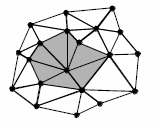
\includegraphics{Figure8-27a}
        \caption*{Locally manifold}\label{fig:Figure8-27a}
    \end{subfigure}
    \hfill
    \begin{subfigure}{0.48\linewidth}
        \centering
        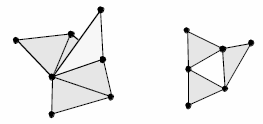
\includegraphics{Figure8-27b}
        \caption*{Locally nonmanifold}\label{fig:Figure8-27b}
    \end{subfigure}%
    \caption{Manifold and nonmanifold surface topology. If the local neighborhood around a vertex is topologically a 2D disk (i.e., a small disk can be placed on the surface without tearing or overlapping), then the surface is manifold at that vertex.}
    \label{fig:Figure8-27}
\end{figure}

Before proceeding we need to define some terms from topology. \emph{Manifold topology} describes a region surrounding a point that is topologically connected. That is, a region around the point is topologically equivalent to a small ``disk'' (in two-dimensions) or ``ball'' (in three-dimensions). Topology that is not manifold is termed \emph{nonmanifol}d. Examples of manifold and nonmanifold geometry are shown in Figure \ref{fig:Figure8-27}.

\begin{figure}[!htb]
    \centering
    \begin{subfigure}{0.24\linewidth}
        \centering
        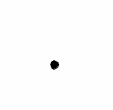
\includegraphics[width=\linewidth]{Figure8-28a}
        \caption*{0D point}\label{fig:Figure8-28a}
    \end{subfigure}
    \hfill
    \begin{subfigure}{0.24\linewidth}
        \centering
        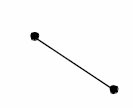
\includegraphics[width=\linewidth]{Figure8-28b}
        \caption*{1D line}\label{fig:Figure8-28b}
    \end{subfigure}%
    \hfill
    \begin{subfigure}{0.24\linewidth}
        \centering
        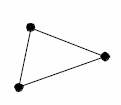
\includegraphics[width=\linewidth]{Figure8-28c}
        \caption*{2D triangle}\label{fig:Figure8-28c}
    \end{subfigure}%
    \hfill
    \begin{subfigure}{0.24\linewidth}
        \centering
        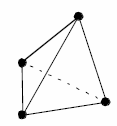
\includegraphics[width=\linewidth]{Figure8-28d}
        \caption*{3D tetrahedron}\label{fig:Figure8-28d}
    \end{subfigure}%
    \caption{Simplices of dimension three and lower.}
    \label{fig:Figure8-28}
\end{figure}

There are some simple rules we can use to decide whether a surface or region approximated with cells is manifold or nonmanifold. In two dimensions, if every edge of a two-dimensional cell is used by exactly one other cell, than the surface is locally manifold. In three dimensions, if every face of a three-dimensional cell is used by exactly one other cell, than the region is locally manifold.

We also will use the term simplex on some occasions. A simplex of dimension n is the convex region defined by a set of n+1 independent points. A vertex, line, triangle, and tetrahedron are simplices of dimension 0, 1, 2, and 3, respectively as shown in Figure \ref{fig:Figure8-28}.

\subsection{Cell Operations}

Cell operations return information about the topology of a cell. Typically, we want to know the topological order of the cell or the topology of the cell boundary.

Given a cell $C_i$ of topological dimension $d$, the cell is (implicitly) composed of boundary cells of topological order $d-1$ and lower. For example, a tetrahedron is composed of four two-dimensional triangles, six one-dimensional edges, and four zero-dimensional vertices. Cell operations return information about the number of boundary cells of a particular topological dimension, as well as the ordered list of points that define each bounding cell.

\begin{figure}[!htb]
    \centering
    \begin{subfigure}{0.48\linewidth}
        \centering
        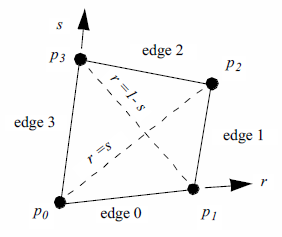
\includegraphics[width=\linewidth]{Figure8-29}
        \caption*{}\label{fig:Figure8-29a}
    \end{subfigure}
    \hfill
    \begin{subfigure}{0.48\linewidth}
    \begin{equation*}
        \begin{array}{lll}
        \text{edge}\: 0 &:& r > s\: and\: r < l - s \\ \\
        \text{edge}\: 1 &:& r > s\: and\: r > l - s \\ \\
        \text{edge}\: 2 &:& r < s\: and\: r > l - s \\ \\
        \text{edge}\: 3 &:& r < s\: and\: r < l - s \\ \\
    \end{array}
    \end{equation*}
    \end{subfigure}%
    \caption{Closest boundary cell operation for quadrilateral cell.}
    \label{fig:Figure8-29}
\end{figure}


Another useful cell operation returns the closest boundary cell of dimension $d-1$ given the parametric coordinates of the cell. This operation ties the geometry to the topology of the cell, as compared to the parametric coordinate system, which ties the topology to the geometry. The closest boundary cell operation is implemented by partitioning each cell into various regions, as illustrated in Figure \ref{fig:Figure8-29}. To determine the closest boundary cell we need only to identify the parametric region that the point lies in, and then return the appropriate boundary cell.

Another useful cell operation is cell decomposition into simplices. Every cell can be decomposed into a collection of simplices. By doing so, and by operating on the simplex decomposition rather than the cell itself, we can create algorithms that are independent of cell type. For example, if we want to intersect two datasets of varied cell type, without simplex decomposition we would have to create methods to intersect every possible combination of cells. With simplex decomposition, we can create a single intersection operation that operates on only the limited set of simplices. The significant advantage of this approach is that as new cells are added to the visualization system, only the cell object (including its method for simplex decomposition) must be implemented, and no other objects need be modified.

\subsection{Dataset Operations}

Dataset operations return information about the topology of a dataset or topological information about the adjacency of cells. Typical operations include determining the neighbors of a cell or returning a list of all cells that use a particular point.

We can formalize the adjacency operations by continuing the discussion of ``Cell Types'' on page \pageref{sec:cell_types}. Adjacency methods are used to obtain information about the neighbors of a cell. A neighbor of a particular cell $C_i$ is simply a cell that shares one or more points in common with $C_i$. A vertex neighbor is a neighbor that shares one or more vertices. An edge neighbor is a neighbor that shares one or more edges. A face neighbor is a cell that shares vertices that define one of the faces of the cell. Note that a face neighbor is also an edge neighbor, and an edge neighbor is also a vertex neighbor.

The adjacency operators are simple set operations. For a particular cell $C_i$ defined by points

\begin{equation}\label{eq:8.24}
C_i = \lbrace p_1, p_2, \ldots, p_n \rbrace = P
\end{equation}
\myequations{Points list.}

and a point list $\overrightarrow{P} = (\overrightarrow{p_1}, \overrightarrow{p_2}, ..., \overrightarrow{p_n})$  with $P \subset P$, where $P$ typically corresponds to the points defining a boundary cell of $C_i$; the neighbors of $C_i$ are the adjacency set A(C, P). The adjacency set is simply the intersection of the use sets for each point, excluding the cell $C_i$.

\begin{equation}\label{eq:8.25}
A(C_i, \overline{P}) = \left(\bigcap_{i} U(\overline{p}_i)\right) - C_i\end{equation}
\myequations{Intersection of the use sets for each point.}

The adjacency set represents a variety of useful information. In a manifold object represented by a polyhedra, for example, each polygon must have exactly one edge neighbor for each of its edges. Edges that have no neighbors are boundary edges; edges that have more than one edge neighbor represent nonmanifold topology. Datasets that consist of three-dimensional cells (e.g., unstructured grids) are topologically consistent only if, for each cell, there is exactly one face neighbor for each face. Faces that have no neighbors are on the boundary of the dataset. More than one face neighbor implies that the neighbors are self-intersecting (in 3D space).

\section{Searching}
\label{sec:searching}
Searching is an operation to find the cell containing a specified point $p$, or to locate cells or points in a region surrounding $p$.
Algorithms requiring this operation include streamline generation, where we need to find the starting location within a cell; probing, where the data values at a point are interpolated from the containing cell; or collision detection, where cells in a certain region must be evaluated for intersection.
Sometimes (e.g., image datasets), searching is a simple operation because of the regularity of data. However, in less structured data, the searching operation is more complex.

To find the cell containing $p$, we can use the following naive search procedure.
Traverse all cells in the dataset, finding the one (if any) that contains $p$.
To determine whether a cell contains a point, the cell interpolation functions are evaluated for the parametric coordinates $(r,s,t)$.
If these coordinates lie within the cell, then $p$ lies in the cell.
The basic assumption here is that cells do not overlap, so that at most a single cell contains the given point $p$.
To determine cells or points lying in the region surrounding $p$, we can traverse cells or points to see whether they lie within the region around $p$.
For example, we can choose to define the region as a sphere centered at $p$.
Then, if a point or the points composing a cell lie in the sphere, the point or cell is considered to be in the region surrounding $p$.

These naive procedures are unacceptable for all but the smallest datasets, since they are of order O(n), where n is the number of cells or points. To improve the performance of searching, we need to introduce supplemental data structures to support spatial searching. Such structures are well-known and include MIP maps, octrees, kd-trees, and binary sphere trees (see ``Bibliographic Notes'' on page \pageref{bibnote:advanced_data_representation} at the end of this chapter).

The basic idea behind these spatial search structures is that the search space is subdivided into smaller parts, or buckets. Each bucket contains a list of the points or cells that lie within it. Buckets are organized in structured fashion so that constant or logarithmic time access to any bucket is possible. For example, if we assign a portion of 2D Euclidean space into a grid of n by m buckets, the location of p in a particular bucket can be determined with two subtractions and two divisions: a constant time access. Similarly, the location of p in a nonuniformly subdivided octree is determined in logarithmic time, since recursive insertion into octant children is required. Once the bucket is found, the search is then limited to the points or cells contained within it. In a properly designed spatial search structure, the number of points or cells in a bucket is a small portion of the total number of cells and less than a fixed value. Thus, the time to search within a bucket can be bounded by a fixed constant. The result is that introducing spatial search structures reduces search times to a maximum $O(log\: n)$, or better yet $O(n)$.

We have two options when applying spatial search structures. We may insert points into the search structure, or we may insert cells, depending on the application. There are advantages and disadvantages to both approaches. Inserting cells into buckets is not a trivial operation. In general, cells are arbitrarily oriented and shaped, and will not fit completely into a single bucket. As a result, cells often span multiple buckets. To reliably determine whether a cell is in a bucket requires geometric intersection tests, a costly operation. Another approach is to use the bounding box\index{bounding box} of a cell to decide which bucket(s) a cell belongs in. We only need to intersect the bounding box with a bucket to determine whether the cell may belong in the bucket. Unfortunately, even though this operation is generally fast, often cells are associated with buckets even though they may not actually lie inside them, wasting (in large models) memory resources and extra processing time.

\begin{figure}[!htb]
    \centering
    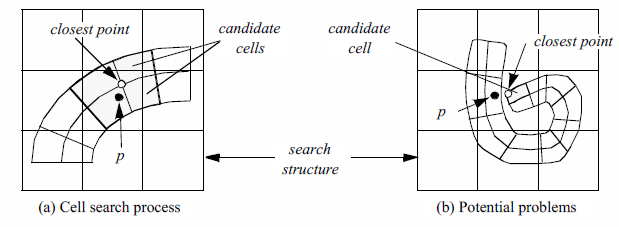
\includegraphics[width=0.98\textwidth]{Figure8-30}\\
    \caption{Using search structure (containing points) to find cells. (a) Points are associated with appropriate bucket. Point p is used to index into bucket, and closest point(s) $p_i$ is found. Cells using $p_i$ are evaluated for the cell containing $p$. (b) Sometimes closest points $p_i$ are not used by cells containing $p$.}\label{fig:Figure8-30}
\end{figure}

Inserting points into a search structure is easier because points can be uniquely placed into a bucket. Inserting points also allows us to search for both points and cells. Cells can be found by using $p$ to index into the appropriate bucket. The closest point(s) $p_i$ to $p$ are then located. Using the topological adjacency operator to retrieve the cells using points $p_i$i, we can then search these cells for the cell containing $p$. This procedure must be used with caution, however, since the closest points may not be used by the cells containing $p$ (Figure\ref{fig:Figure8-30}).

\section{Cell / Line Intersection}
\index{cell!intersection with line|(}

An important geometric operation is intersection of a line with a cell. This operation can be used to interactively select a cell from the rendering window, to perform ray-casting for rendering, or to geometrically query data.

\begin{figure}[!htb]
    \centering
    \begin{subfigure}{0.32\linewidth}
        \centering
        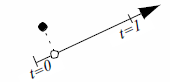
\includegraphics[width=0.98\linewidth]{Figure8-31a}
        \captionsetup{singlelinecheck=off}
        \caption*{\centering{\textbf{Vertex}}
        \begin{itemize}[leftmargin=*]
            \itemsep0em
            \item project point onto ray
            \item distance to line must be within tolerance
            \item $t \in [0,1]$
        \end{itemize}
        }
        \label{fig:Figure8-31a}
    \end{subfigure}
    \hfill
    \begin{subfigure}{0.32\linewidth}
        \centering
        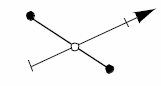
\includegraphics[width=0.98\linewidth]{Figure8-31b}
        \captionsetup{singlelinecheck=off}
        \caption*{\centering{\textbf{Line}}
        \begin{itemize}[leftmargin=*]
            \itemsep0em
            \item 3D line intersection
            \item distance between linese must be within tolerance
            \item $s, t \in [0,1]$
        \end{itemize}
        }
        \label{fig:Figure8-31b}
    \end{subfigure}%
    \hfill
    \begin{subfigure}{0.32\linewidth}
        \centering
        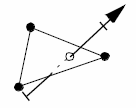
\includegraphics[width=0.98\linewidth]{Figure8-31c}
        \captionsetup{singlelinecheck=off}
        \caption*{\centering{\textbf{Triangle}}
        \begin{itemize}[leftmargin=*]
            \itemsep0em
            \item line/plane intersection
            \item intersection point must lie in triangle
            \item $t \in [0,1]$
        \end{itemize}
        }
        \label{fig:Figure8-31c}
    \end{subfigure}%
    \hfill
    \begin{subfigure}{0.32\linewidth}
        \centering
        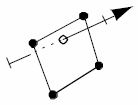
\includegraphics[width=\linewidth]{Figure8-31d}
        \captionsetup{singlelinecheck=off}
        \caption*{\centering{\textbf{Quadrilateral}}
        \begin{itemize}[leftmargin=*]
            \itemsep0em
            \item line/plane intersection
            \item intersection point must lie in quadrilateral
            \item $t \in [0,1]$
        \end{itemize}
        }
        \label{fig:Figure8-31d}
    \end{subfigure}%
    \begin{subfigure}{0.32\linewidth}
        \centering
        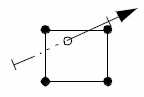
\includegraphics[width=\linewidth]{Figure8-31e}
        \captionsetup{singlelinecheck=off}
        \caption*{\centering{\textbf{Pixel}}
        \begin{itemize}[leftmargin=*]
            \itemsep0em
            \item line/plane intersection
            \item intersection point must lie in pixel (uses efficient in/out test)
            \item $t \in [0,1]$
        \end{itemize}
        }
        \label{fig:Figure8-31e}
    \end{subfigure}
    \hfill
    \begin{subfigure}{0.32\linewidth}
        \centering
        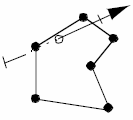
\includegraphics[width=\linewidth]{Figure8-31f}
        \captionsetup{singlelinecheck=off}
        \caption*{\centering{\textbf{Polygon}}
        \begin{itemize}[leftmargin=*]
            \itemsep0em
            \item line/plane intersection
            \item intersection point must lie in polygon (uses ray casting for polygon in/out)
            \item $t \in [0,1]$
        \end{itemize}
        }
        \label{fig:Figure8-31f}
    \end{subfigure}%
    \hfill
    \begin{subfigure}{0.32\linewidth}
        \centering
        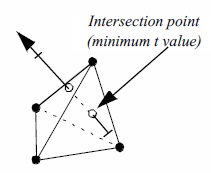
\includegraphics[width=\linewidth]{Figure8-31g}
        \captionsetup{singlelinecheck=off}
        \caption*{\centering{\textbf{Tetrahedron}}
        \begin{itemize}[leftmargin=*]
            \itemsep0em
            \item intersect each (triangle) face
            \item $t \in [0,1]$
        \end{itemize}
        }
        \label{fig:Figure8-31g}
    \end{subfigure}%
    \begin{subfigure}{0.32\linewidth}
        \centering
        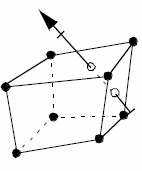
\includegraphics[width=\linewidth]{Figure8-31h}
        \captionsetup{singlelinecheck=off}
        \caption*{\centering{\textbf{Hexahedron}}
        \begin{itemize}[leftmargin=*]
            \itemsep0em
            \item intersect each (quadrialteral) face
            \item since face may be nonplanar, project previous result onto hexahedron surface
            \item $t \in [0,1]$
        \end{itemize}
        }
        \label{fig:Figure8-31h}
    \end{subfigure}
    \hfill
    \begin{subfigure}{0.32\linewidth}
        \centering
        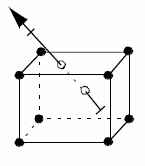
\includegraphics[width=\linewidth]{Figure8-31i}
        \captionsetup{singlelinecheck=off}
        \caption*{\centering{\textbf{Hexahedron}}
        \begin{itemize}[leftmargin=*]
            \itemsep0em
            \item intersect each (pixel) face
            \item $t \in [0,1]$
        \end{itemize}
        }
        \label{fig:Figure8-31i}
    \end{subfigure}%
    \caption{Summary of line/cell intersection operations for nine primitive cell types. Line is assumed normalized in parametric coordinate $t$ with $t \in [0,1]$.}
    \label{fig:Figure8-31}
\end{figure}

In the \emph{Visualization Toolkit} each cell must be capable of intersecting itself against a line. Figure \ref{fig:Figure8-31} summarizes these operations for the nine linear primary cell types supported by VTK. (Intersections on composite cells are implemented by intersecting each primitive cell in turn). Note that the procedure for intersecting higher order cells is the same.

Line/cell intersection for 0D, 1D, and 2D cells follows standard approaches. Intersection against 3D cells is difficult. This is because the surfaces of these cells are described parametrically and are not necessarily planar. For example, to intersect a line with a tetrahedron, we can intersect the line against the four triangular faces of the tetrahedron. Hexahedron, however, may have non-planar faces. Thus, we cannot intersect the line against six quadrilateral, planar faces. Instead, we use line/face intersection as an initial guess, and project the intersection point onto the surface of the cell. This produces an approximate result, but is accurate enough for most applications.
\index{cell!intersection with line|)}

\section{Scalars and Colors}
\index{color!as scalar data|(}

There is a close correspondence between scalar data and colors. We touched on this in ``Color Mapping'' on page \pageref{subsec:color_mapping}, where we saw how to use a color table to map scalar values into a color specification (i.e., red, green, blue, and alpha, or RGBA). There are cases, however, when we want to circumvent this mapping process. Such cases occur when color data is supplied instead of scalar data.

A common example occurs in imaging. Recall that an image is a regular, two-dimensional array of points. The points define pixels, which in turn form a two-dimensional image dataset. Images are frequently stored as a pair of dimensions along with data values. The data values may be one of black and white (e.g., a bitmap), grayscale, or color (e.g., a pixmap). Bitmaps and gray-scale images can be directly cast into the form of single-values scalar data, and we can use our earlier approach. Pixmaps, however, consist of (at a minimum) three values per pixel of red, green, and blue. (Sometimes, a fourth alpha opacity value may also be included.) Thus, pixmaps cannot be directly cast into scalar form.

To accommodate color data, conversions between multicomponent color data and single-valued scalars must be defined. Each class must act as if it were a scalar: that is, a request for data at a particular point must return a single scalar value. This allows us to use standard scalar visualization techniques such as contouring or warping. Thus a mapping from RGB or RGBA color coordinates to a single scalar value is required.

The simplest conversion is to select one of n components in a color tuple and use that as the scalar value. Another common mapping returns the luminance Y of a color. Given three components, RGB, the luminance is

\begin{equation}\label{eq:8.26}
Y = 0.30 R + 0.59 G + 0.11 B\end{equation}
\myequations{RGB luminance.}

If the color includes transparency, RGBA, the luminance is
\begin{equation}\label{eq:8.27}
Y = A(0.30 R + 0.59 G + 0.11 B)
\end{equation}
\myequations{RGBA luminance.}

Using this abstraction allows us to treat single--valued scalars and scalars consisting of multivalued colors the same. The end result is that we can mix both types of scalar data into our visualization networks.
\index{color!as scalar data|)}

\section{Special Techniques for Image Data}
\label{sec:special_techniques_for_image_data}

A significant attraction of using 2-- and 3--dimensional image data is the speed and simplicity of computation. In this section, we will explore specific techniques that exploit the special regular topology and geometry of image data.

\subsection{Coordinate Transformation}
\index{image data!coordinate transformation|(}

\begin{figure}[!htb]
    \centering
    \begin{subfigure}{0.48\linewidth}
        \centering
        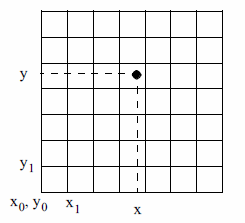
\includegraphics[width=\linewidth]{Figure8-32}
        \caption*{}\label{fig:Figure8-32a}
    \end{subfigure}
    \hfill
    \begin{subfigure}{0.48\linewidth}
    \begin{equation*}
        \begin{array}{lll}
        i &=& \text{floor}(\dfrac{x - x_0}{x_1 - x_0}) \\ \\
        j &=& \text{floor}(\dfrac{y - y_0}{y_1 - y_0}) \\ \\
        k &=& \text{floor}(\dfrac{z - z_0}{z_1 - z_0}) \\ \\
    \end{array}
    \end{equation*}
    \begin{equation*}
        \begin{array}{lll}
        r &=& \text{frac}(\dfrac{x - x_0}{x_1 - x_0}) \\ \\
        s &=& \text{frac}(\dfrac{y - y_0}{y_1 - y_0}) \\ \\
        t &=& \text{frac}(\dfrac{z - z_0}{z_1 - z_0}) \\ \\
    \end{array}
    \end{equation*}
    \end{subfigure}%
    \caption{Closest boundary cell operation for quadrilateral cell.}
    \label{fig:Figure8-32}
\end{figure}


Given a point $p$ we can find the structured coordinates by performing three division operations (Figure \ref{fig:Figure8-32}). Taking the integer floor function yields the structured coordinates. Taking the fractional part of the result yields the parametric coordinates of the cell. We can then use Equation \ref{eq:8.3} to convert to dataset coordinates.
\index{image data!coordinate transformation|)}

\subsection{Derivative Computation}
\index{image data!derivatives|(}

\begin{figure}[!htb]
	\floatbox[{\capbeside\thisfloatsetup{capbesideposition={right,center},capbesidewidth=0.4\textwidth}}]{figure}[\FBwidth]
	{\caption{Using finite differences to compute derivatives on image data.}\label{fig:Figure8-33}}
	{\includegraphics[width=0.6\textwidth]{Figure8-33}}
\end{figure}


Because the image dataset is oriented parallel to the coordinate x, y, and z axes, and because the spacing of points in each of these directions is regular, finite difference schemes can be used to compute partial derivatives at the cell points. Referring to Figure \ref{fig:Figure8-33}, we see that central differences can be used in each of the three directions according to the equation:

\begin{equation}\label{eq:8.28}
\begin{array}{lll}
g_x &=& \dfrac{d(x_0 + \Delta x_0, y_0, z_0) - d(x_0 - \Delta x_0, y_0, z_0)}{2 \Delta x_0} \\ \\
g_y &=& \dfrac{d(x_0, y_0 + \Delta y_0, z_0) - d(x_0, y_0 - \Delta y_0, z_0)}{2 \Delta y_0} \\ \\
g_z &=& \dfrac{d(x_0, y_0, z_0 + \Delta z_0) - d(x_0, y_0, z_0 - \Delta z_0)}{2 \Delta z_0}
\end{array}
\end{equation}
\myequations{Computing image data derivatives.}

(Note that at the boundary of the dataset, one-sided differences may be used.) We can use these equations to compute derivatives within the cell as well. We simply compute the derivatives at each cell point from Equation \ref{eq:8.28}, and then use the cell interpolation functions to compute the derivative at the point inside the cell.
\index{image data!derivatives|)}

\subsection{Topology}
\index{image data!topology|(}

Structured datasets lend themselves to efficient topological operations (i.e., both image data and structured grids). Given a cell id, it is possible to determine vertex, edge, or face neighbors using simple constant time operations. First, given the cell id in a three-dimensional structured dataset, we use a combination of division and modulo arithmetic to compute the structured coordinates

\begin{equation}\label{eq:8.29}
\begin{array}{lll}
i &=& \text{id}\ \text{modulo}\ (n_x - 1) \\ \\
j &=& \left( \dfrac{\text{id}}{n_x - 1} \right)\ \text{modulo}\ (n_y - 1) \\ \\
k &=& \dfrac{\text{id}}{\left((n_x - 1)(n_y - 1)\right)}
\end{array}
\end{equation}
\myequations{Computing the structured coordinates.}

Face neighbors are determined by incrementing one of the $i$, $j$, or $k$ indices. Edge neighbors are determined by incrementing any two indices, while vertex neighbors are found by incrementing all three indices. Care must be taken while incrementing to insure that the indices fall in the range

\begin{equation}\label{eq:8.30}
\begin{array}{l}
0 \leq i < n_x - 1 \\
0 \leq j < n_y - 1 \\
0 \leq k < n_z - 1
\end{array}
\end{equation}
\myequations{Range for the indices.}

An attempt to index outside these ranges indicates that the neighbor in question does not exist.
\index{image data!topology|)}

\subsection{Searching}
\label{subsec:searching}
\index{image data!searching|(}

Given a point $p = (x, y, z)$ we can determine the cell containing $p$ by using the equations given in Figure \ref{fig:Figure8-32}. These equations generate the structured coordinates $(i, j, k)$, which can then be converted to cell id (i.e., dataset coordinates) using Equation 8-3.

To find the closest point to $p$, we compute the structured coordinates by rounding to the nearest integer value (instead of using the floor function). Thus,

\begin{equation}\label{eq:8.31}
\begin{array}{lll}
i = \text{int}\left( \dfrac{x-x_0}{x_1 - x_0} \right) \\ \\
j = \text{int}\left( \dfrac{y-y_0}{y_1 - y_0} \right) \\ \\
k = \text{int}\left( \dfrac{z-z_0}{z_1 - z_0} \right)
\end{array}
\end{equation}
\myequations{Finding the closest point to $p$ using structured coordinates.}
\index{image data!searching|)}

\section{Putting It All Together}

In this section we will finish our earlier description of an implementation for unstructured data. We also define a high-level, abstract interface for cells and datasets. This interface allows us to implement the general (i.e., dataset specific) algorithms in the \emph{Visualization Toolkit}. We also describe
implementations for color scalars, searching and picking, and conclude with a series of examples to demonstrate some of these concepts.

\subsection{Unstructured Topology}

In Chapter 5: \nameref{chap:basic_data_representation} we described data representations for the unstructured dataset types vtkPolyData and vtkUnstructuredGrid. Close examination of this data structure reveals that operations to retrieve topological adjacency are inefficient. In fact, to implement any operation to retrieve vertex, edge, or face neighbors requires a search of the cell array, resulting in $O(n)$ time complexity. This is unacceptable for all but the smallest applications, since any algorithm traversing the cell array and retrieving adjacency information is at a minimum$ O(n^2)$.

The reason for this inefficiency is that the data representation is a ``downward'' hierarchy (Figure \ref{fig:Figure8-34}(b)). That is, given a cell we can quickly determine the topological features lower in the topological hierarchy such as faces, edges, and points. However, given a face, edge, or point we must search the cell array to determine the owning cells. To improve the efficiency of this data representation, we must introduce additional information into the hierarchy that allows ``upward'' hierarchy traversal (similar to that shown in Figure \ref{fig:Figure8-34}(a)).


\begin{figure}[!htb]
    \centering
    \begin{subfigure}{0.32\linewidth}
        \centering
        \includegraphics{Figure8-34a}
        \caption{Hierarchical topological
        structure}\label{fig:Figure8-34a}
    \end{subfigure}
    \hfill
    \begin{subfigure}{0.32\linewidth}
        \centering
        \includegraphics{Figure8-34b}
        \caption{Basic unstructured data representation}\label{fig:Figure8-34b}
    \end{subfigure}%
    \hfill
    \begin{subfigure}{0.32\linewidth}
        \centering
        \includegraphics{Figure8-34c}
        \caption{Full unstructured data representation}\label{fig:Figure8-34c}
    \end{subfigure}%
    \caption{Enhancing hierarchical unstructured data representation. (a) Conventional topological hierarchy for geometric model. (b) Basic unstructured data hierarchy. (c) Full unstructured data hierarchy. By introducing upward references from points to cells, the unstructured data hierarchy may be efficiently traversed in both directions, and is more compact than conventional topological hierarchies.}
    \label{fig:Figure8-34}
\end{figure}

\begin{figure}[!htb]
    \centering
    \includegraphics[width=0.98\textwidth]{Figure8-35}\\
    \caption{Complete unstructured data representation including link lists. There are m cells and n points. The n structures in the link list are lists of cells that use each vertex. Each link list is variable in length.}\label{fig:Figure8-35}
\end{figure}


The solution to this problem is to extend the unstructured data structure with cell links. The cell links array is a list of lists of cells that use each point and corresponds to the upward links of Figure \ref{fig:Figure8-34}(c). The cell links array transforms the hierarchical structure of Figure \ref{fig:Figure5-13} into a ring structure. Cells reference their composing points, and points in turn reference the cells that use them. The full unstructured data structure is shown in Figure \ref{fig:Figure8-35}.The cell links array is in fact an implementation of the use sets of Equation \ref{eq:5.1}. We can use this equation to compute adjacency operation in constant time, if the maximum number of cells using a point is much smaller than the number of points in a dataset. To see this, we refer to Equation \ref{eq:8.25} and see that the adjacency operations consist of a finite number of set intersections. Each operation is an intersection of the link lists for each point. If the number of cells in each link list is ``small'', then the intersection operation can be bounded by a fixed constant in time, and the total operation can be considered a constant time operation.

There are several important characteristics of this data representation.

\begin{itemize}

\item The cell links array is an extension of the basic unstructured data representation. As a result, we can defer the construction of the cell links until they are required. Often the cell links are never needed and require no computer resources to compute or store.

\item Building the cell links is a linear $O(n)$ operation. Each cell is traversed and for every point that the cell uses, the list of using cells for that point is extended to include the current cell. Building the cell links is only needed once as an initialization step.

\item The data representation is compact relative to other topology representation schemes (e.g., the winged--edge structure and the radial--edge structures \cite{Baumgart74} \cite{Weiler88}). These other data structures contain explicit representation of intermediate topology such as edges, loops, faces, or special adjacency information such as adjacent edges (winged--edge structure) or extensive ``use'' descriptions (radial--edge structure). The compactness of representation is particularly important for visualization, since the data size is typically large.

\end{itemize}

The unstructured data structure in the \emph{Visualization Toolkit} is implemented using the four classes vtkPoints (and subclasses), vtkCellArray, vtkCellTypes, and vtkCellLinks. The building of this data structure is incremental. At a minimum, the points and cells are represented using vtkPoints and vtkCellArray. If random access or extra type information is required, then the object vtkCellTypes is used. If adjacency information is required, an instance of the class vtkCellLinks is created. These operations are carried out behind the scenes, and generally do not require extra knowledge by the application programmer.

\clearpage

\subsection{Abstract Interfaces}

With the completion of Chapter 5: \nameref{chap:basic_data_representation} and Chapter 8: \nameref{chap:advanced_data_representation}, we can summarize the abstract interface for cells, datasets, and the point data attributes. These pseudo-code descriptions encapsulate the core functionality of the classes vtkDataSet, vtkCell, and vtkPointData, and their subclasses. All algorithms presented in this text can be implemented using combinations of these methods.

\begin{description}
\item[Dataset Abstraction.\index{abstraction!dataset|(}\index{dataset!abstraction|(}] The dataset is the central data representation in VTK. Datasets are composed of one or more cells and points. Associated with the points are attribute data consisting of scalars, vectors, normals, texture coordinates, and tensors.
    \setlist[description]{font=\normalfont,style=nextline}
    \begin{description}

    \item[\texttt{type = GetDataObjectType()}]
    Return the type of dataset (e.g., vtkPolyData, vtkImageData, vtkStructuredGrid, vtkRectilinearGrid, or vtkUnstructuredGrid).

    \item[\texttt{numPoints = GetNumberOfPoints()}]
    Return the number of points in the dataset.

    \item[\texttt{numCells = GetNumberOfCells()}]
    Return the number of cells in the dataset.

    \item[\texttt{GetPoint(ptId,x)}]
    Given a point id, return the (x,y,z) coordinates of the point.

    \item[\texttt{cell = GetCell(cellId)}]
    Given a cell id, return a pointer to a cell object.

    \item[\texttt{type = GetCellType(cellId)}]
    Return the type of the cell given by cell id.

    \item[\texttt{GetCellTypes(types)}]
    Return a list of types of cells that compose the dataset.

    \item[\texttt{cells = GetPointCells(ptId)}]
    Given a point id, return the cells that use this point.

    \item[\texttt{GetCellPoints(cellId, ptIds)}]
    Given a cell id, return the point ids (e.g., connectivity list) defining the cell.

    \item[\texttt{GetCellNeighbors(cellId, ptIds, neighbors)}]
    Given a cell id and a list of points composing a boundary face of the cell, return the neighbors of that cell sharing the points.

    \item[\texttt{cellId = FindCell(x, cell, cellId, tol2, subId, pcoords, weights)}] 
    Given a coordinate value x, an initial search cell defined by cell and cellId, and a tolerance measure (squared), return the cell id and sub-id of the cell containing the point and its interpolation function weights. The initial search cell is used to speed up the search process when the position x is known to be near the cell. If no cell is found, cellId < 0 is returned.

    \item[\texttt{pointData = GetPointData()}]
    Return a pointer to the object maintaining point attribute data. This includes scalars, vectors, normals, tensors, and texture coordinates, as well as any other data arrays that the field carries.

    \item[\texttt{cellData = GetCellData()}]
    Return a pointer to the object maintaining cell attribute data. This includes scalars, vectors, normals, tensors, and texture coordinates, as well as any other data arrays that the field carries.

    \item[\texttt{bounds = GetBounds()}]
    Get the bounding box of the dataset.

    \item[\texttt{length = GetLength()}]
    Return the length of the diagonal of the bounding box of the dataset.

    \item[\texttt{center = GetCenter()}]
    Get the center of the bounding box of the dataset.

    \item[\texttt{range = GetScalarRange()}]
    A convenience method to return the (minimum, maximum) range of the scalar attribute data associated with the dataset.

    \item[\texttt{dataSet = NewInstance()}]
    Make a copy of the current dataset. A ``virtual'' constructor. (Typically, reference counting methods are used to copy data.)

    \item[\texttt{CopyStructure(dataSet)}]
    Update the current structure definition (i.e., geometry and topology) with the supplied dataset.
    \end{description}
\index{abstraction!dataset|)}\index{dataset!abstraction|)}

\item[Cell Abstraction.\index{abstraction!cell|(}\index{cell!abstraction|(}] Cells are the atomic structures of VTK. Cells consist of a topology, defined by a sequence of ordered point ids, and a geometry, defined by point coordinates. The cell coordinate consists of a cell id, a subcell id, and a parametric coordinate. The subid specifies a primary cell that lies within a composite cell such as a triangle strip. Cell edges and faces are defined implicitly from the topology of the cell.
    \setlist[description]{font=\normalfont,style=nextline}
    \begin{description}

    \item[\texttt{type = GetCellType()}]
    Return the type of the cell. Must be one of the twelve VTK cell types (or the empty cell type).

    \item[\texttt{dim = GetCellDimension()}]
    Return the topological definition of the cell.

    \item[\texttt{order = GetInterpolationOrder()}]
    Return the degree of the interpolating polynomial of the cell. (The twelve cell types are all degree 1; cells added in the future may be of higher-order.)

    \item[\texttt{numberPoints = GetNumberOfPoints()}]
    Return the number of points that define the cell.

    \item[\texttt{points = GetPoints()}]
    Return a list of point ids defining the cell.

    \item[\texttt{numberEdges = GetNumberOfEdges()}]
    Return the number of edges in the cell.

    \item[\texttt{edge = GetEdge(i)}]
    Given an edge id ( 0 ≤ i < numberEdges ) return a pointer to a cell that represents an edge of the cell.

    \item[\texttt{numberFaces = GetNumberOfFaces()}]
    Return the number of faces in a cell.

    \item[\texttt{face = GetFace(i)}]
    Given an face id ( 0 ≤ i < numberFaces ) return a pointer to a cell that represents a face of the cell.

    \item[\texttt{inOutStatus = CellBoundary(subId, pcoords, poindIds)}]
    Given a cell subid and parametric coordinates, return a list of point ids that define the closest boundary face of the cell. Also return whether the point is actually in the cell.

    \item[\texttt{inOutStatus = EvaluatePosition(x, closestPoint, subId, pcoords, weights, dist2)}]
    Given a point coordinate x, return the sub-id, parametric coordinates, and interpolation weights of the cell if x lies inside the cell. The position closestPoint is the closest point on the cell to x (may be the same) and dist2 is the squared distance between them. The method returns an inOutStatus indicating whether x is topologically inside or outside the cell. That is, the point may satisfy parametric coordinate conditions but may lie off the surface of the cell (e.g., point lies above polygon). Use both inOutStatus and dist2 to determine whether point is both topologically and geometrically in the cell.

    \item[\texttt{EvaluateLocation(subId, pcoords, x, weights)}]
    Given a point location (i.e., sub-id and parametric coordinates), return the position x of the point and the interpolation weights.

    \item[\texttt{Contour(value, cellScalars, locator, verts, lines, polys, inputPointData, outputPointData)}]
    Given a contour value and scalar values at the cell points, generate contour primitives (vertices, lines, or polygons with associated points and attribute data values). The points are placed in a locator object (see ``Searching'' on page \pageref{subsec:searching}) which merges coincident points, and the attribute data values are interpolated (along the cell edge) from the inputPointData to the outputPointData.

    \item[\texttt{Clip(value, cellScalars, locator, cells, inputPointData, outputPointData, insideOut)}]
    Given a contour value and scalar values at the cell points, clip the cell to generate new cells of the same topological dimension as the original cell. The points are placed in a locator object (see ``Searching'' on page \pageref{subsec:searching}) which merges coincident points, and the attribute data values are interpolated (or copied) from the inputPointData to the outputPointData. The clipped cells are placed in the cells list.

    \item[\texttt{Derivatives(subId, pcoords, values, dim, derivs)}]
    Given a cell location (i.e., subid and parametric coordinates) and data values at the cell points, return $dim*3$ derivatives (i.e., corresponds to the \emph{x}, \emph{y}, and \emph{z} directions times dimension of data).

    \item[\texttt{inOutStatus = IntersectWithLine(p1, p2, tol, t, x, pcoords, subId)}] 
    Given a finite line defined by the two points p1 and p2 and an intersection tolerance, return the point of intersection x. The parametric coordinate t along the line and cell location at the point of intersection is also returned. Returns a nonzero if intersection occurs.

    \item[\texttt{Triangulate(index, ptIds, points)}]
    Decompose the cell into simplices of dimension equal to the topological cell dimension. The index is an integer that controls the triangulation if more than one triangulation  is possible. The simplices are defined by an ordered list of point ids and their corresponding coordinates.

    \item[\texttt{bounds = GetBounds()}]
    Return the bounding box of the cell.

    \end{description}
\index{abstraction!cell|)}\index{cell!abstraction|)}

\item[Point and Cell Attribute Abstraction.\index{abstraction!dataset attribute|(}\index{dataset attribute!abstraction|(}] Point and cell attribute data is information associated with the points and cells of a dataset. This information consists of scalars, vectors, normals, tensors, and texture coordinates. There is a one-to-one relationship between the points and cells in a dataset and its corresponding point and cell attribute data. For example, a point scalar value at location $100$ is associated with point $id$ $100$.

Many of the methods described below deal with moving data from the input to the output of a filter. Since the possibility exists that new types of attribute data could be added in the future, the details of moving data is hidden as much as possible (i.e., minimize the knowledge that the filter has about specific attribute types). Thus, generic functions like CopyData() allow for copying data from the input to the output without knowing what this data is.
    \setlist[description]{font=\normalfont,style=nextline}
    \begin{description}

    \item[\texttt{CopyScalarsOn() / CopyScalarsOff()}]
    Turn on/off boolean flag controlling copying of scalar data from input to output of filter.

    \item[\texttt{CopyVectorsOn() / CopyVectorsOff()}]
    Turn on/off boolean flag controlling copying of vector data from input to output of filter.

    \item[\texttt{CopyNormalsOn() / CopyNormalsOff()}]
    Turn on/off boolean flag controlling copying of normal data from input to output of filter.

    \item[\texttt{CopyTensorsOn() / CopyTensorsOff()}]
    Turn on/off boolean flag controlling copying of tensor data from input to output of filter.

    \item[\texttt{CopyTextureCoordsOn() / CopyTextureCoordsOff()}]
    Turn on/off boolean flag controlling copying of texture coordinates data from input to output of filter.

    \item[\texttt{CopyAllOn() / CopyAllOff()}]
    Turn on/off all boolean flags controlling copying of all attribute data from input to output of filter.

    \item[\texttt{PassData(pointData)}]
    Transfer all point attribute data (pointData) to the output according to the copy flags listed previously.

    \item[\texttt{CopyAllocate(pointData)}]
    Initialize and allocate storage for point-by-point copy process.

    \item[\texttt{CopyData(pointData, fromId, toId)}]
    Given point data and a specific point id, copy the point attribute data (pointData) to the output point.

    \item[\texttt{InterpolateAllocate(pointData)}]
    Initialize and allocate storage for point-by-point interpolation process.

    \item[\texttt{InterpolatePoint(pointData, toId, ptIds, weights)}]
    Given input point data (pointData) and a list of points and their interpolation weights, interpolate data to the specified output point.

    \item[\texttt{InterpolateEdge(pointData, toId, p1, p2, t)}]
    From an edge defined by the two points p1 and p2, interpolate the pointData at the edge parametric coordinate t and copy the interpolated attribute data to the output point ptId.

    \item[\texttt{NullPoint(int ptId)}]
    Set the data value(s) of the specified output point id to a null value.

    \item[\texttt{SetScalars() / GetScalars()}]
    Set / return scalar data. The GetScalars() method may return a NULL value, in which case the scalars are not defined.

    \item[\texttt{SetVectors() / GetVectors()}]
    Set / return vector data. The GetVectors() method may return a NULL value, in which case the vectors are not defined.

    \item[\texttt{SetNormals() / GetNormals()}]
    Set / return normal data. The GetNormals() method may return a NULL value, in which case the normals are not defined.

    \item[\texttt{SetTensors() / GetTensors()}]
    Set / return tensor data. The GetTensors() method may return a NULL value, in which case the tensors are not defined.

    \item[\texttt{SetTextureCoords() / GetTextureCoords()}]
    Set / return texture coordinate data. The GetTextureCoords() method may return a NULL value, in which case the texture coordinates are not defined.

    \end{description}
\end{description}
\index{abstraction!dataset attribute|)}\index{dataset attribute!abstraction|)}

\subsection{Traversing Intermediate Topology}

The dataset abstraction implemented by VTK provides simple techniques to traverse points and cells. Sometimes we want to traverse intermediate topology such as edges or faces. For example, to identify boundary edges in a triangular mesh we must traverse each edge, counting the number of triangles that use each edge. (Recall that boundary edges are used by just one triangle.) Unfortunately, there is no obvious way to traverse edges. The same problem holds true if we want to traverse the faces of a dataset containing 3D cells.

A simple solution is to traverse each cell and then obtain the edges (or faces) that compose the cell. The problem with this approach is that edges and faces are generally used by more than one cell, resulting in multiple visits to the same face or edge. This may be acceptable in some algorithms, but usually we count on visiting each edge or face only once.

A better solution to this problem is to traverse each cell as before, but only process intermediate topology if the current cell has the smallest cell id. (The current cell is the cell being visited in the traversal process.) To determine whether the current cell has the smallest cell id, we obtain all cells using the intermediate topology. This information can be obtained using the topological adjacency operators described earlier (e.g., Equation \ref{eq:8.25}).

To illustrate this process consider visiting the edges of a triangle mesh. We begin by visiting the first triangle, $t$, and then its edges. For each edge we determine the adjacent triangle(s) (if any) that use the edge. If the id of the adjacent triangle(s) is greater than triangle $t$'s id, or there are no adjacent triangles, then we know to process the current edge. (Of course the first triangle will always have the smallest id  --- but this will change as the traversal proceeds.) We then continue traversing the triangle list for new $t$'s. In this way all the edges of the mesh will be visited.

\subsection{Color Scalar Data}
\index{color!as scalar data!implementation|(}

Multivalued scalar data, or scalars represented by various color representations, are treated specially by the \emph{Visualization Toolkit}. These data arise, for example, when using a color specification to directly control the color of objects rather than mapping a scalar value through a lookup table. (See ``Color Mapping'' on page \pageref{subsec:color_mapping} for more information.)

By default, the mapping of scalars into colors proceeds as follows (vtkMapper and subclasses are responsible for implementing this behavior):
\begin{itemize}

\item If the scalar type is unsigned char with the tuple size ranging between one and four components, the data is considered to be color data.

\item Four component data is assumed to be a RGBA (red--green--blue--alpha transparency) color specification. Three component data is assumed to be a RGB color specification. Two component data is assumed to be a IA (intensity--alpha) representation. Single component data is assumed to be a I (intensity) value.

\item Any other data type, or data with more than four components, is assumed to represent a scalar value. In that case the scalars are mapped through a lookup table to produce colors during the rendering process.

\end{itemize}

It is possible to force unsigned char data to be mapped through a lookup table. The vtkMapper method SetColorModeToMapScalars() forces all data  (regardless of type) to be mapped through the lookup table.
\index{color!as scalar data!implementation|)}

\subsection{Searching}

The \emph{Visualization Toolkit} provides two classes to perform searches for dataset points and cells. These are vtkPointLocator and vtkCellLocator. (Both of these classes are subclasses of vtkLocator, which is an abstract base class for spatial search objects.) vtkPointLocator is used to search for points and, if used with the topological dataset operator GetPointCells(), to search for cells as well. vtkCellLocator is used to search for cells.

vtkPointLocator is implemented as a regular grid of buckets (i.e., same topology and geometry as an image dataset). The number of buckets can be user-specified, or more conveniently, automatically computed based on the number of dataset points. On average, vtkPointLocator provides constant time access to points. However, in cases where the point distribution is not uniform, the number of points in a bucket may vary widely, giving O(n) worst-case behavior. In practice this is rarely a problem, but adaptive spatial search structures (e.g., an octree) may sometimes be a better choice.


\begin{figure}[!htb]
	\floatbox[{\capbeside\thisfloatsetup{capbesideposition={left,center},capbesidewidth=0.4\textwidth}}]{figure}[\FBwidth]
	{\caption{Determining closest point to $p$ in vtkPointLocator. Initial search in bucket results in point $a$. Search must extend beyond local bucket as a function of search radius $R$, resulting in point $b$.}\label{fig:Figure8-36}}
	{\includegraphics[width=0.6\textwidth]{Figure8-36}}
\end{figure}

Determining closest point to a point $p$ using vtkPointLocator (as well as other spatial search structures) is a three-step process. In the first step, the bucket containing $p$ is found using the appropriate insertion scheme. (For vtkPointLocator this is three divisions to determine bucket indices $(i, j, k)$.) Next, the list of points in this bucket is searched to determine the closest point. However, as Figure \ref{fig:Figure8-36} shows, this may not be the true closest point, since points in neighboring buckets may be closer. Consequently, a final search of neighboring buckets is necessary. The search distance is a function of the distance to the current closest point. Once all neighbors within this distance are searched, the closest point is returned.

\begin{figure}[!htb]
    \centering
    \begin{subfigure}{0.48\linewidth}
        \centering
        \includegraphics[width=\linewidth]{Figure8-37}
        \caption*{}\label{fig:Figure8-37a}
    \end{subfigure}
    \hfill
    \begin{subfigure}{0.48\linewidth}
    Cell list structure (Union)
    \begin{lstlisting}[caption={}, numbers=none, frame=none]
    if parent octant:
      IN/OUT flag
     if terminal octant:
       list of cells
    \end{lstlisting}
    level of octree, $l$
    number of terminal octants, $n_T$
    \begin{equation*}
        n_T = 8^l
    \end{equation*}
    number of octants, $n_O$
    \begin{equation*}
        n_O = \sum_{i = 0}^i 8^i
    \end{equation*}
    number of parents, $n_p$
    \begin{equation*}
        n_p = n_O - n_T
    \end{equation*}
    \end{subfigure}%
    \caption{ Structure of spatial search structure vtkCellLocator. The data structure represents a uniformly subdivided octree.}
    \label{fig:Figure8-37}
\end{figure}

vtkCellLocator is implemented as a uniformly subdivided octree with some peculiar characteristics (Figure \ref{fig:Figure8-37}). Conventional octree representations use upward parent and downward children pointers to track parent and children octants. Besides the required list of entities (i.e., points or cells) in each octant, additional information about octant level, center, and size may also be maintained. This results in a flexible structure with significant overhead. The overhead is the memory resources to maintain pointers, plus the cost to allocate and delete memory.

In contrast, vtkCellLocator uses a single array to represent the octree. The array is divided into two parts. The first part contains a list of parent octants, ordered according to level and octant child number. In the second part are the terminal, or leaf octants. The terminal octants are ordered on a regular array of buckets, just the same as vtkLocator. The terminal octants contain a list of the entities inside the octant. The parent octants maintain a value indicating whether the octant is empty, or whether something is inside it. (Both types of information are represented in the same portion of the octant structure.) Because the octree is uniformly subdivided, parent-child relationships, as well as octant locations, can be computed quickly using simple division operations.

The advantage of this structure is that memory can be allocated and deleted quickly. In addition, insertion into the octree is exactly the same as with vtkLocator, and is simpler than conventional octrees. The parent octants provide quick culling capability, since their status (empty or nonempty) allows us to stop certain types of search operations. On the downside, because the octree is uniformly subdivided, this structure is wasteful of memory resources if the data is nonuniformly distributed.

Our experience with the search structures described here is that they work well for many types of visualization data. However, if your data is non-uniform, you may want to implement your own special search classes.


\subsection{Picking}
\label{subsec:picking}

\begin{figure}[!htb]
	\floatbox[{\capbeside\thisfloatsetup{capbesideposition={right,center},capbesidewidth=0.4\textwidth}}]{figure}[\FBwidth]
	{\caption{The picking hierarchy in VTK. All subclasses of vtkAbstractPropPicker return the picked instance of vtkProp. The information is returned as a vtkAssemblyPath. The assembly path is necessary because some props may exist in an assembly hierarchy. The classes vtkWorldPointPicker and vtkPropPicker are hardware accelerated picking classes. All others use software ray casting.}\label{fig:Figure8-38}}
	{\includegraphics[width=0.6\textwidth]{Figure8-38}}
\end{figure}


The Visualization Toolkit provides a variety of classes to perform actor (or vtkProp), point, cell, and world point picking ( Figure \ref{fig:Figure8-38}).

All pickers are subclasses of vtkAbstractPicker which defines the basic pick interface. The user must specify a selection point in display coordinates for a specified instance of vtkRenderWindow and invoke the Pick() method. At a minimum, the class must return an $x-y-z$ pick position in world coordinates. It is possible to limit the pick candidates to a list of vtkProps (the PickList). The class also invokes the StartPickEvent\index{events!StartPickEvent}, PickEvent\index{events!PickEvent}, and EndPickEvent\index{events!EndPickEvent} events that are invoked prior to picking, during picking, and after picking, respectively.

Classes that can return information indicating which vtkProp they have picked are subclasses of vtkAbstractPropPicker. After the pick operation, vtkAbstractPropPicker returns a vtkAssemblyPath. The assembly path is an ordered list of instances of vtkProp and possibly associated 4x4 transformation matrices. The path represents a concatenated hierarchy of assembly nodes if an assembly has been defined (see ``Assemblies and Other Types of vtkProp'' on page \pageref{subsubsec:assemblies_vtkprop} for more information about props and assemblies).

\begin{figure}[!htb]
    \centering
    \begin{subfigure}{0.32\linewidth}
        \centering
        \includegraphics[width=\linewidth]{Figure8-39a}
        \caption{vtkPicker}\label{fig:Figure8-39a}
    \end{subfigure}
    \hfill
    \begin{subfigure}{0.32\linewidth}
        \centering
        \includegraphics[width=\linewidth]{Figure8-39b}
        \caption{vtkPointPicker}\label{fig:Figure8-39b}
    \end{subfigure}%
    \hfill
    \begin{subfigure}{0.32\linewidth}
        \centering
        \includegraphics[width=\linewidth]{Figure8-39c}
        \caption{vtkCellPicker}\label{fig:Figure8-39c}
    \end{subfigure}%
    \hfill
    \begin{subfigure}{0.48\linewidth}
        \centering
        \includegraphics[width=\linewidth]{Figure8-39d}
        \caption{vtkWorldPointPicker}\label{fig:Figure8-39d}
    \end{subfigure}%
    \hfill
    \begin{subfigure}{0.48\linewidth}
        \centering
        \includegraphics[width=\linewidth]{Figure8-39e}
        \caption{vtkPropPicker}\label{fig:Figure8-39e}
    \end{subfigure}%
    \caption{Summary of picking operations. The top three pick classes (a)-(c) use software ray casting. The bottom two pick classes (d)-(e) use hardware acceleration.}
    \label{fig:Figure8-39}
\end{figure}

The object vtkPicker intersects a ray defined from camera position to a screen (i.e., pixel) coordinate against the bounding box of all pickable and nontransparent vtkProp3D's. (A vtkProp is pickable if its Pickable instance variable is true.) The result of the vtkPicker pick operation is to return a list of the vtkProp3D's whose bounding box is intersected. The prop closest to the camera position is also returned.

The object vtkPointPicker intersects the ray against the points defining each vtkProp3D, and returns the point coordinate closest to the camera position, as well as the vtkProp3D that the point belongs to. Since screen resolution prevents precise selection of a point, a tolerance around the ray must be specified. The tolerance is expressed as a fraction of the rendering window size. (Rendering window size is measured across the window diagonal.) Points must lie within this tolerance to be picked.

The object vtkCellPicker intersects the ray with the cells defining each vtkProp3D, and returns the point of intersection, as well as the vtkProp3D that the cell belongs to. If you are trying to select a cell belonging to a particular vtkProp3D, vtkCellPicker is the object to use because it performs surface (or cell) intersection. Unfortunately, vtkCellPicker is the slowest of the pickers because of greater computational requirements.

The class vtkWorldPointPicker returns the $(x,y,z)$ coordinate value of a pick in the rendering window. To determine this information, it combines the display $(x,y)$ values with the z-buffer depth values. Of all the pickers this is the fastest, but it cannot determine the actual cell, point or vtkProp that is selected since it is not a subclass of vtkAbstractPropPicker. (Note: on some systems \emph{z}--buffer operations are inoperative and this object will not function properly.)

By default picking is performed with the class vtkPropPicker. This class uses hardware-accelerated picking --- so it is generally faster than software based picking. Unlike the other hardware accelerated class (vtkWorldPointPicker), it returns the instance of vtkProp that was picked as well as the $(x,y,z)$ world coordinate value

Figure \ref{fig:Figure8-39} summarizes the five concrete picking classes. Picking is built into the vtkRenderWindowInteractor class using the ``p'' key (see ``Introducing vtkRenderWindowInteractor'' on page \pageref{subsec:introducing_vtkRenderWindowInteractor}). By default a vtkPropPicker is created and used, but you are free to specify your own picker type.

\subsection{Examples}

To conclude this section, we will examine how some of the dataset, cell, and point attribute operations are used. These operations tend to be used by class developers. You will not need to use them if you build applications by constructing visualization pipelines with existing filters.

\subsubsection{Find Free Edges}

\begin{figure}[!htb]
    \centering
    \begin{subfigure}{0.48\linewidth}
        \centering
        \includegraphics[width=\linewidth]{Figure8-40a}
        \caption{Linear}\label{fig:Figure8-40a}
    \end{subfigure}
    \hfill
    \begin{subfigure}{0.48\linewidth}
        \centering
        \includegraphics[width=\linewidth]{Figure8-40b}
        \caption{Rotational}\label{fig:Figure8-40b}
    \end{subfigure}%
    \caption{Depiction of linear and rotational extrusion.}
    \label{fig:Figure8-40}
\end{figure}

In our first example we will take a peek inside the filter vtkLinearExtrusionFilter. This filter implements the following modelling operation. Given a polygonal mesh, extrude the mesh in a given direction, constructing a ``skirt'' or ``walls'' from the free edges. If the polygonal example is a single square, the result of this operation is a cube. Or, if the polygonal data consists of a single line, the result of the operation is a quadrilateral. A point will generate a line as shown in Figure \ref{fig:Figure8-40}(a).

Recall that free edges are edges used by only one polygon. We can determine this information using the dataset topology operation GetCellEdgeNeigbors(). We use Equation \ref{eq:8.25} and the two points defining the edge of the polygon to determine the adjacency set (i.e., the polygons sharing this edge). If no other polygon uses this edge, then the edge is extruded to generate a triangle strip. The C++ pseudo code is as follows.

\begin{lstlisting}[language=C++, caption={Determining free edges.}]
for (cellId=0; cellId < numCells; cellId++)
  {
  cell = mesh->GetCell(cellId);
  if ((dim=cell->GetCellDimension()) == 0)
  //create lines from points
  else if ( dim == 1 )
  // create strips from lines
  else if ( dim == 2 ) // create strips from boundary edges
    {
    numEdges = cell->GetNumberOfEdges();
    for (i=0; i<numEdges; i++)
      {
      edge = cell->GetEdge(i);
      for (j=0; j<(edge->GetNumberOfPoints()-1); j++)
        {
        p1 = edge->PointIds->GetId(j);
        p2 = edge->PointIds->GetId(j+1);
        mesh.GetCellEdgeNeighbors(cellId, p1, p2, cellIds);
        if ( cellIds->GetNumberOfIds() < 1 )
          {
          //generate triangle strip
          }
        } //for each subedge
      } //for each edge
    } //for each polygon or triangle strip
  } //for each cell
\end{lstlisting}

\begin{figure}[!htb]
    \centering
    \begin{subfigure}{0.96\linewidth}
        \centering
        \includegraphics[width=.96\linewidth]{Figure8-41a}
        \caption{Linearly extruded fonts to show letter frequency in text.(\href{https://lorensen.github.io/VTKExamples/site/Cxx/Visualization/AlphaFrequency/}{AlphaFrequency.cxx} or \href{https://lorensen.github.io/VTKExamples/site/Python/Visualization/AlphaFrequency/}{AlphaFrequency.py})}\label{fig:Figure8-41a}
    \end{subfigure}
    \hfill
    \begin{subfigure}{0.48\linewidth}
        \centering
        \includegraphics[width=.96\linewidth]{Figure8-41b}
        \caption{Rotationally symmetric objects.(\href{https://lorensen.github.io/VTKExamples/site/Cxx/Modelling/Bottle/}{Bottle.cxx} or \href{https://lorensen.github.io/VTKExamples/site/Python/Modelling/Bottle/}{Bottle.py})}\label{fig:Figure8-41b}
    \end{subfigure}%
    \hfill
    \begin{subfigure}{0.48\linewidth}
        \centering
        \includegraphics[width=.96\linewidth]{Figure8-41c}
        \caption{Rotation in combination with linear displacement and radius variation.(\href{https://lorensen.github.io/VTKExamples/site/Cxx/Modelling/Spring/}{Spring.cxx} or \href{https://lorensen.github.io/VTKExamples/site/Python/Modelling/Spring/}{Spring.py})}\label{fig:Figure8-41c}
    \end{subfigure}%
    \caption{Models created using linear and rotational extrusion.}
    \label{fig:Figure8-41}
\end{figure}

This same approach is used in the vtkRotationalExtrusionFilter (Figure \ref{fig:Figure8-40}(b)). The difference between these two functions is that the type of motion is rotational as compared to linear (vtkLinearExtrusionFilter). These two filters can be used to perform some nifty modelling operations. Linear extrusion can be used to create bar charts with arbitrary cross sections, or to sweep out three-dimensional fonts. The rotational extrusion filter can be used to create rotationally symmetric objects such as bottles or wine glasses. Examples of these techniques are shown in Figure \ref{fig:Figure8-41}.

\subsubsection{Find Cells}

In this example we combine picking and a topological operation to select cells sharing a common point. Specifically, we use vtkPointPicker and the topological dataset operation GetPointCells(). Figure \ref{fig:Figure8-42} depicts this operation. We have also included a fragment of C++ code implementing this procedure. Note that this procedure will work for any dataset type, even if the geometry is implicitly defined (e.g., vtkImageData).

\begin{figure}[!htb]
    \centering
    \begin{subfigure}{0.48\linewidth}
        \centering
        \includegraphics[width=.96\linewidth]{Figure8-42a}
        \caption*{}\label{fig:Figure8-42a}
    \end{subfigure}
    \hfill
    \begin{subfigure}{0.48\linewidth}
        \centering
        \includegraphics[width=.96\linewidth]{Figure8-42b}
        \caption{Selected cells}\label{fig:Figure8-42b}
    \end{subfigure}%
    \hfill
    \begin{subfigure}{0.96\linewidth}
        \centering
        \begin{lstlisting}[language=C++,  caption={}, numbers=none, frame=none]
        sphereActor->SetPosition(picker->GetPickPosition());
        if ( picker->GetPointId() >= 0 )
          {
          cout << "Point id: " << picker->GetPointId() << "\n";
          cellsActor->VisibilityOn();
          plateActor->VisibilityOff();
          cells->Initialize();
          cells->Allocate(100);
          cells->SetPoints(plateOutput->GetPoints());
          plateOutput->GetPointCells(picker->GetPointId(), cellIds);
          for (i=0; i < cellIds->GetNumberOfIds(); i++)
            {
            cellId = cellIds->GetId(i);
            plateOutput->GetCellPoints(cellId, ptIds);
            cells->InsertNextCell(plateOutput->GetCellType(cellId), ptIds);
            }
          }
        else
          {
          cellsActor->VisibilityOff();
          plateActor->VisibilityOn();
          }
        renWin->Render();
        \end{lstlisting}
        \caption{C++ code probe.cxx}\label{fig:Figure8-42c}
    \end{subfigure}%
    \caption{Creating a point probe. Visualization network shown in diagram above. C++ code shows inner loop of vtkProbeFilter and resulting image for combustor data (probe.cxx).}
    \label{fig:Figure8-42}
\end{figure}

The most difficult part of this procedure is the picking process. The selection point must be specified in pixel coordinates. The vtkPointPicker converts these coordinates into world and then dataset coordinates using the renderer in which the pick occurred. (The renderer uses the transformation matrix of its active camera to perform coordinate transformation.)

The picking process is conveniently managed in vtkRenderWindowInteractor. This object allows the specification of functions to execute just before picking and just after picking (i.e., ``AddObserver StartPickEvent'' and ``AddObserver EndPickEvent''). Using this facility we can define a postpicking function to retrieve the point id and then execute the GetPointCells() operation. This process is shown in Figure \ref{fig:Figure8-42}.

\subsubsection{Point Probe}
\label{subsec:examples.point_probe}

In this example we will show how to build a point probe using the dataset and cell operations described in this chapter. A point probe is defined as follows. Given a $(x,y,z)$ point coordinate, find the cell coordinates (i.e., cell id, subcell id, and parametric coordinates) and the interpolation weights. Once the interpolation weights are found, we can then compute local data values at $(x,y,z)$.

\begin{figure}[!htb]
    \centering
    \begin{subfigure}{0.96\linewidth}
        \centering
        \includegraphics[width=.96\linewidth]{Figure8-43a}
        \caption{Original data}\label{fig:Figure8-43a}
    \end{subfigure}
    \hfill
    \begin{subfigure}{0.96\linewidth}
        \centering
        \begin{lstlisting}[language=C++,  caption={}, numbers=none, frame=none]
        //
        // Loop over all input points, interpolating source data
        //
        for (ptId=0; ptId < numPts; ptId++)
          {
          // Get the xyz coordinate of the point in the input dataset
          x = input->GetPoint(ptId);
          // Find the cell that contains xyz and get it
          cell = source->FindAndGetCell(x,NULL,-1,tol2,subId,pcoords,weights);
          if (cell)
            {
            // Interpolate the point data
            outPD->InterpolatePoint(pd,ptId,&(cell->PointIds),weights);
            }
          else
            {
            outPD->NullPoint(ptId);
            }
          }
        \end{lstlisting}
        \caption{C++ code (pickCells.cxx)}
    \end{subfigure}%
    \caption{Models created using linear and rotational extrusion.}
    \label{fig:Figure8-43}
\end{figure}

The point probe is implemented using the dataset operation FindCell(). This method requires a point specified in global coordinates (our $(x,y,z)$ value) and a tolerance. The tolerance is often necessary because of numerical precision or when picking near the surface of 3D cells, or on 0D, 1D, and 2D cells. The FindCell() operation returns the information we require, plus the interpolation weights of the cell containing our point probe. To determine the data value at our probe point, we need to retrieve the data values on the cell points. We can then use the interpolation functions of Equation \ref{eq:8.4} to determine the probe scalar value.

Figure \ref{fig:Figure8-43} depicts this process and includes C++ code. In the example we use the combustor dataset with the objects vtkCursor3D, vtkProbeFilter, and vtkGlyph3D. The purpose of the cursor is to control the position of the probe point. The class vtkProbeFilter performs the probing  operation just described. (This filter has been generalized so that it can handle more than one input point.) vtkGlyph3D is used to place an oriented, scaled cone at the cursor focal point. This gives us visual feedback about the scalar and vector quantities at the probe. Of course, we can extract numeric values and display them to the user if this is important.

\section{Chapter Summary}

Three important visualization coordinate systems are the world, dataset, and structured coordinate systems. The world coordinate system is an x--y--z Cartesian three-dimensional space. The dataset coordinate system consists of a cell id, subcell id, and parametric coordinates. The structured coordinate system consists of $(i,j,k)$ integer indices into a rectangular topological domain.

Visualization data is generally in discrete form. Interpolation functions are used to obtain data at points between the known data values. Interpolation functions vary depending on the particular cell type. The form of the interpolation functions are weighting values located at each of the cells points. The interpolations functions form the basis for conversion from dataset to global coordinates and vice versa. The interpolation functions also are used to compute data derivatives.

Topological operators provide information about the topology of a cell or dataset. Obtaining neighboring cells to a particular cell is an important visualization operation. This operation can be used to determine whether cell boundaries are on the boundary of a dataset or to traverse datasets on a cell-by-cell basis.

Because of the inherent regularity of image datasets, operations can be efficiently implemented compared to other dataset types. These operations include coordinate transformation, derivative computation, topological query, and searching.

\section{Bibliographic Notes}
\label{bibnote:advanced_data_representation}

Interpolation functions are employed in a number of numerical techniques. The finite element method, in particular, depends on interpolation functions. If you want more information about interpolation functions refer to the finite element references suggested below \cite{Cook89} \cite{Gallagher75} \cite{Zienkiewicz87}. These texts also discuss derivative computation in the context of interpolation functions.

Visualizing higher-order datasets is an oepn research issue. While \cite{Schroeder06} describes one approach, methods based on GPU programs are emerging. Other approaches include tailored algorithms for a particular cell type.

Basic topology references are available from a number of sources. Two good descriptions of topological data structures are available from Weiler \cite{Weiler86} \cite{Weiler88} and Baumgart \cite{Baumgart74}. Weiler describes the radial-edge structure. This data structure can represent manifold and nonmanifold geometry. The winged-edge structure described by Baumgart is widely known. It is used to represent manifold geometry. Shephard \cite{Shephard88} describes general finite element data structures  --- these are similar to visualization structures but with extra information related to analysis and geometric modelling.

There are extensive references regarding spatial search structures. Samet \cite{Samet90} provides a general overview of some. Octrees were originally developed by Meagher \cite{Meagher82} for 3D imaging. See \cite{Williams83}, \cite{Bentley75}, and \cite{Quinlan94} for information about MIP maps, kd-trees, and binary sphere trees, respectively.

\printbibliography


\section{Exercises}

\begin{figure}[!htb]
    \centering
    \begin{subfigure}{0.32\linewidth}
        \centering
        \includegraphics[width=.98\linewidth]{Figure8-44a}
        \caption{}\label{fig:Figure8-44a}
    \end{subfigure}
    \hfill
    \begin{subfigure}{0.32\linewidth}
        \centering
        \includegraphics[width=.98\linewidth]{Figure8-44b}
        \caption{}\label{fig:Figure8-44b}
    \end{subfigure}%
    \hfill
    \begin{subfigure}{0.32\linewidth}
        \centering
        \includegraphics[width=.98\linewidth]{Figure8-44c}
        \caption{}\label{fig:Figure8-44c}
    \end{subfigure}%
    \hfill
    \begin{subfigure}{0.48\linewidth}
        \centering
        \includegraphics[width=.65\linewidth]{Figure8-44d}
        \caption{}\label{fig:Figure8-44d}
    \end{subfigure}%
    \hfill
    \begin{subfigure}{0.48\linewidth}
        \centering
        \includegraphics[width=.65\linewidth]{Figure8-44e}
        \caption{}\label{fig:Figure8-44e}
    \end{subfigure}%
    \caption{Exercise figures.}
    \label{fig:Figure8-44}
\end{figure}

\begin{enumerate}

\item Given a volume of dimensions $5 \times 10 \times 15$ with origin $(1.0, 2.0,3.0)$ and voxel spacing $(0.5, 0.5, 1.0)$.
    \begin{enumerate}

    \item Compute minimum point position.

    \item Compute maximum point position.

    \item For cell id 342, compute cell minimum point position and maximum point position.

    \item What points (list ids) define cell id 342?

    \item Given point specified in structured coordinates as $(i, j, k) = (3, 6, 4)$ ;$(r, s, t) = (0.1, 0.2, 0.5)$, compute global coordinates.

    \end{enumerate}

\item Compute global coordinates and interpolation weights for the points specified in dataset coordinates (refer to Figure \ref{fig:Figure8-44}(a-d)).
    \begin{enumerate}

    \item Line with $r = 0.5$.

    \item Triangle with $(r, s) = (0.25, 0.33)$.

    \item Voxel with $(r, s, t) = (0.25, 0.33, 0.5)$.

    \end{enumerate}

\item Compute parametric coordinates for cells shown in Figure \ref{fig:Figure8-44}(a-d).
    \begin{enumerate}

    \item Line with $(x, y, z) = (0.3, 0.6, 0.9)$.

    \item Triangle with $(x, y, z) = (0.5, 0.25, 0.0)$.

    \item Voxel with $(x, y, z) = (0.5, 0.4, 2.0)$.

    \end{enumerate}

\item Given the line shown in Figure \ref{fig:Figure8-44}(a), if scalar data values are $(s_0, s_1) = (0.0, 0.25)$, what are the derivatives in the $x, y, z$ directions?

\item Refer to Figure \ref{fig:Figure8-44}(d) and let the numbers indicate cell ids and the letters indicate point ids.
    \begin{enumerate}

    \item List the cells using point A.

    \item List the cells using point B.

    \item List cells using edge (A, B). How does this list correspond to your answers in parts a) and b) above?

    \end{enumerate}

\item Refer to Figure \ref{fig:Figure8-44}(e).
    \begin{enumerate}

    \item How many boundary faces are there?

    \item How many ``internal'' faces?

    \end{enumerate}

\item Describe a procedure to intersect two finite lines. How does tolerance value come into play?

\item Describe a procedure to intersect a line and triangle. Are there special characteristics of a triangle that can be used to speed this operation?

\item Compare memory requirements for the three unstructured grid data structures shown in Figure \ref{fig:Figure8-34}. Assume that two cells use each face, four faces use each edge, and six edges use each vertex (i.e., a structured dataset).

\item Using the abstract cell and dataset interface, write a program to compute
    \begin{enumerate}

    \item number of points in a dataset,

    \item number of cells in a dataset,

    \item number of edges in a dataset,

    \item number of faces in a dataset.

    \end{enumerate}

\item Given a volume of dimensions $5 \times 10 \times 15$.
    \begin{enumerate}

    \item How many internal faces are there (i.e. used by two voxels)?

    \item How many boundary faces are there (i.e., used by one voxel)?

    \end{enumerate}

\item Write a general extrusion filter that sweeps an object along a path to construct a new surface. Assume that the path is defined by a sequence of transformation matrices. Can you think of a way to prevent self-intersection?

\end{enumerate}
